\documentclass[dissertation.tex]{subfiles}
\begin{document}

\chapter[Signatures of Survival Processes in Pancreas Cancer][Survival Signatures]{Signatures of Survival Processes in Pancreas Cancer}
\label{chap:signatures}

\emph{Thesis: Specific molecular processes control survival of patients with resectable \acrlong{PDAC}, and  these processes can be identified using \acrlong{GEX} data.}

\paragraph{Summary}Very little is known regarding the biological processes that control the survival of patients with \gls{PDAC}, the most common and aggressive form of pancreas cancer.  The range of relative patient survival times that is observed in practice is not well explained by extrinsic factors such as age at diagnosis, and perhaps instead reflects differences in the biological processes operating within each tumour.  Recent molecular profiling work~\cite{Collisson2011} has identified possible molecular subtypes within the previously homogenous group of \gls{PDAC}, but these subtypes have not achieved the maturity or clinical application of those in breast cancer, and their discovery and validation has been hampered by ad-hoc methodology, and the lack of large, well-curated cohorts of \gls{PDAC} samples.  The recently-compiled \gls{APGI} cohort contains the largest group of clinically annotated \gls{PDAC} samples, with accompanying \gls{GEX} and high-quality follow-up data, in the world.  It presents a unique opportunity to apply modern techniques for prognostic signature identification to the discovery of biological processes that drive the clinical course of pancreas cancer.  These signatures may find application as prognostic tools in their own right, but more importantly can supply much-needed information on the fundamental biology of the one common cancer that has, to date, been almost entirely refractory to all the tools of modern molecular medicine.

\section{Introduction}
Despite extensive research, \gls{PDAC} remains a poorly-understood disease.  Recent genomic profiling has revealed the genetic alterations that accompany the cancer~\cite{Biankin2012}, and a huge number of prognostic factors are known~\cite{Harsha2009}, but these findings have shed little light on the fundamental disease processes at work in individual tumours.  This is a consequence of genetic and biomarker data being poorly-suited for understanding the biological state of a cell: although genetic alterations are central to the etiology of cancer, they give incomplete information on the pathways and systems actually active in a given tumour, and biomarkers supply non-causal readouts of cell state that are difficult to trace back to underlying biological processes.

Sitting between the regulatory function of transcription control, and the effector function of protein expression, \gls{GEX} data integrate information from all aspects of cell condition, including genetic alterations, signalling pathway activity, and metabolic status.  As such, it is unsurprising that \gls{GEX} data are superior indicators of cell state, better than all other high-throughput measurement methods, such as protein expression or genetic alterations~\cite{Ray2014}.  However, the involvement of \gls{GEX} with so many biological inputs is also a weakness: typical differential expression studies will identify many hundreds of transcripts that vary between disease states, and the deconvolution of this complex set of hundreds of effects back to a small number of causative molecular processes remains challenging.

Disease \gls{GEX} profiling studies have largely refrained from attempting to infer the state of a few molecular processes from the many hundreds of differentially-expressed genes identified.  A number of factors are likely to have contributed to this reluctance: deconvolution methods require relatively large sets of high-quality measurements~\cite{MacCallum1999}, early techniques were poorly-suited to the particular requirements of the \gls{GEX} deconvolution problem, and the signature databases that assist the assignation of a biological annotation to the output from a deconvolution calculation (for example, the \acrshort{MSIGDB}~\cite{Subramanian2005}) are only now reaching maturity, with some areas of biology still under-represented.

A simple synthetic example illustrates the problem and process of \gls{GEX} deconvolution, and the character of solutions produced by both classical and modern techniques.  Consider a group of samples, each of which is in one of three distinct biological states: state A, state B, and an intermediate state.  Which state a sample is in affects the expression of two genes, gene 1, and gene 2: state A is associated with higher gene 2 expression than gene 1 expression; state B with higher gene 1 expression than gene 2; and the intermediate state with low expression for both genes (\fref{fig:sigs-example-matrixfactor-data}).  From the figure it is apparent that samples lie along two lines in transcription space; these lines I term metagenes.

Accurately knowing the metagenes at work within a biological system considerably simplifies reasoning about transcription within the system.  In the example of \fref{fig:sigs-example-matrixfactor-data}, state A is associated with high metagene 1, state B with high metagene 2, and the transition state with low scores of both.  Additionally, the loadings of genes on the metagenes themselves (the directions of the metagene arrows) provides information on transcriptional control within the system: metagenes define the axes along which cell state must move, and so provide a simpler and more accurate representation of cell state than the full set of gene expression measurements.  Metagenes can also be considered to capture co-expressed modules of genes, with likely biological significance.  The advantages of a metagene-centric perspective to interpreting \gls{GEX} become increasingly apparent as more genes are considered, and when thousands of genes are measured per sample, deconvolving the highly complex patterns of expression of thousands of genes, to only tens of metagenes, represents a powerful reduction in complexity.  However, in practical use deconvolution methods must operate in thousand dimensional spaces, rather than the two dimensions in this example, and the computational and methodological complexities involved, as well as the poor results yielded by traditional approaches, have limited the application of \gls{GEX} deconvolution.

\begin{figure}[!htbp]
\centering
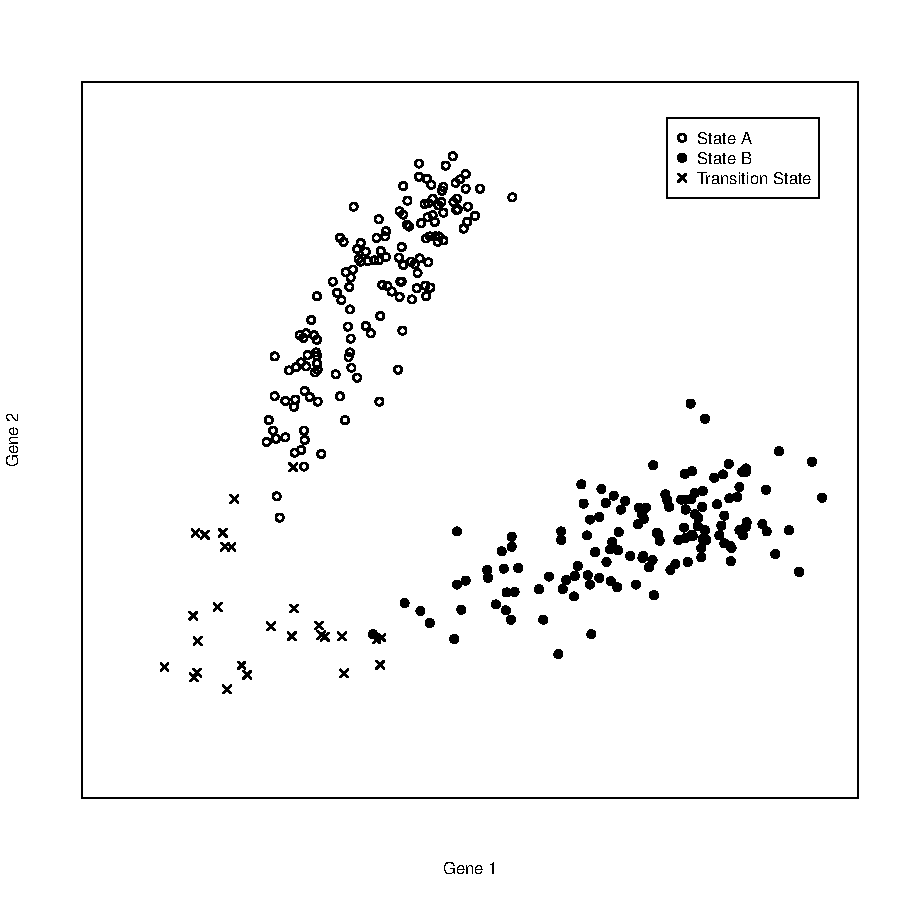
\includegraphics[width=.7\linewidth]{analysis/biosurv/reports/PCA_ICA_NMF_comparison/figure/plots-1}
\caption[Illustration of the gene deconvolution problem]{The gene deconvolution problem.  Shown are the hypothetical expression levels of two genes across three biological states, where each point represents the gene expression of a single sample in one of the three biological states.  State A (hollow circles) is characterised by gene 2 $>$ gene 1; state B (solid circles) by gene 1 $>$ gene 2; and the intermediate state (crosses) by low levels of both genes.  The challenge of gene deconvolution is to automatically infer, from unlabelled data (ie state is unknown), the dominant lines of gene expression (metagenes) along which most samples lie.}\label{fig:sigs-example-matrixfactor-data}
\end{figure}

A number of techniques from the field of matrix factorization have been applied to the \gls{GEX} deconvolution problem, first \gls{PCA}~\cite{Alter2000}, then \gls{ICA}~\cite{Liebermeister2002}, and more recently various forms of \gls{NMF}~\cite{Brunet2004}.  A number of reports have highlighted the unsuitability of \gls{PCA} for \gls{GEX} deconvolution, and the relative superiority of \gls{ICA}~\cite{Lee2003, Saidi2004, Teschendorff2007}; this is primarily due to the \gls{PCA} requirement that metagenes be orthogonal~\cite{Lewicki2000}, a situation that is not supported by our knowledge of biology, and results in bizarre artefacts such as \gls{PCA} metagenes not actually being aligned with the expression pattern of any sample (\fref{fig:sigs-example-matrixfactor-methods-pca}).  Although the results from \gls{ICA} are more interpretable than those from \gls{PCA}, they still do not consider that \gls{GEX} is a non-negative process: it is impossible to have a concentration of mRNA that is less than zero, and therefore for best interpretability we wish metagenes to have non-negative `expression' as well.  \gls{ICA} does not produce solutions satisfying this requirement, and more importantly its non-Gaussianity objective is not necessarily optimal for \gls{GEX} deconvolution (\fref{fig:sigs-example-matrixfactor-methods-ica}), reducing its ultimate utility.  \gls{NMF} techniques have the potential to produce excellent \gls{GEX} decompositions (\fref{fig:sigs-example-matrixfactor-methods-nmf}), but are relatively new methods that have very high computational requirements, and often require careful tuning, making their effective application challenging.

\begin{figure}[!htbp]
  \centering
  \subbottom[\texorpdfstring{\acrshort{PCA}}{PCA}]{
    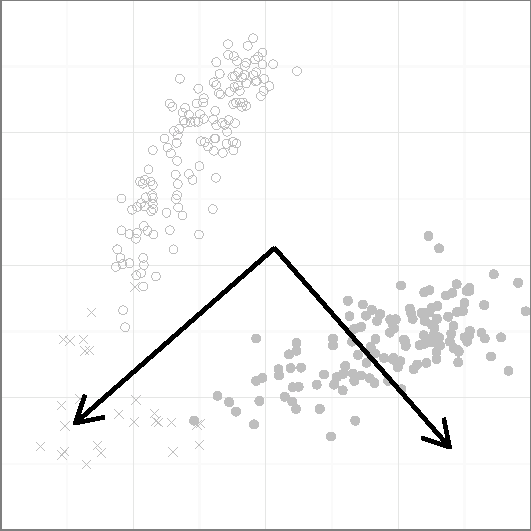
\includegraphics[width=.3\textwidth]{analysis/biosurv/reports/PCA_ICA_NMF_comparison/figure/smallplots-1}
    \label{fig:sigs-example-matrixfactor-methods-pca}}
  \subbottom[\texorpdfstring{\acrshort{ICA}}{ICA}]{
    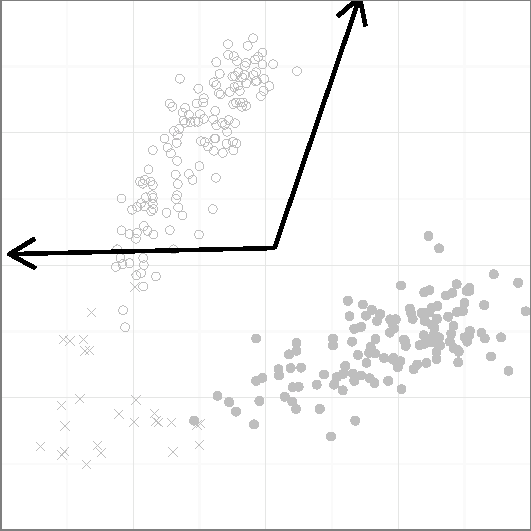
\includegraphics[width=.3\textwidth]{analysis/biosurv/reports/PCA_ICA_NMF_comparison/figure/smallplots-2}
    \label{fig:sigs-example-matrixfactor-methods-ica}}
  \subbottom[\texorpdfstring{\acrshort{NMF}}{NMF}]{
    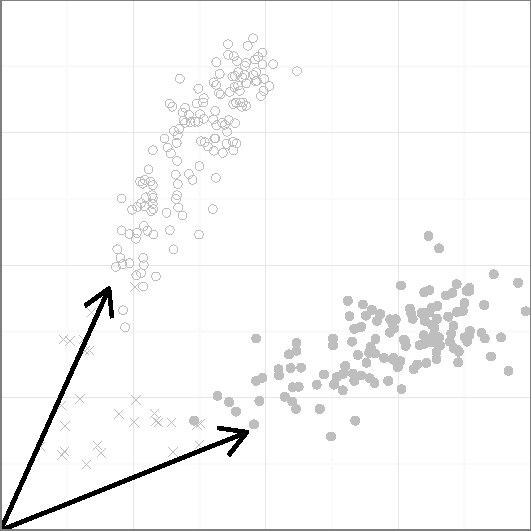
\includegraphics[width=.3\textwidth]{analysis/biosurv/reports/PCA_ICA_NMF_comparison/figure/smallplots-3}
    \label{fig:sigs-example-matrixfactor-methods-nmf}}
  \caption[Comparison of \texorpdfstring{\acrshort{GEX}}{GEX} deconvolution techniques]{\gls{NMF} produces a more accurate \gls{GEX} decomposition than either \gls{PCA} or \gls{ICA}.  Metagenes found by each method are shown as arrows.  \gls{PCA} (panel a) produces metagenes that don't match the expression pattern seen in any sample; these metagenes do not have a ready biological interpretation.  \gls{ICA} (panel b) accurately identifies one metagene, but the inappropriateness of the non-Gaussianity criterion for these data leads to an incorrect estimate of the other; although this solution is better than that of \gls{PCA}, not all metagenes align well with biology.  \gls{NMF} (panel c) provides the best deconvolution; the metagenes identified closely match the expression patterns observed, and reflect the true structure of co-expression within the samples.}\label{fig:sigs-example-matrixfactor-methods}
\end{figure}

In addition to the general technical challenges of \gls{GEX} deconvolution, issues particular to pancreas cancer significantly complicate attempts to identify molecular processes at work within the tumours.  Pancreas cancer is challenging to sample, and mRNA in the tissue degrades rapidly once extracted, complicating sample collection.  Additionally, a feature of \gls{PDAC} is the presence of a dense desmoplastic stromal reaction throughout the tumour, that is formed by genetically normal patient stroma cells~\cite{Mahadevan2007}.  The fraction of tumour cells that are actually cancerous varies by more than 10-fold between tumours~\cite{Biankin2012}, meaning that without careful correction, gene expression profiles are dominated by stromal cell fraction signals, and not true differential expression within a cell type.  Microdissection has been used to separate cancer cells from surrounding stroma in order to simplify analysis~\cite{Collisson2011}, but current thought in the field is that the stroma in \gls{PDAC} is an essential and enabling, if not in itself neoplastic, component of the tumour~\cite{Mahadevan2007}, and that the examination of cancer cell expression in isolation ignores the likely important interplay between the two major synergistic components of a tumour: transformed epithelial cells, and genetically normal stroma.

Due to these challenges to \gls{GEX} deconvolution of \gls{PDAC}, to date only one study (by Collisson \emph{et al}, published in 2011) has reported a breakdown of \gls{PDAC} \gls{GEX} into a small number of biological modules~\cite{Collisson2011}.  This study examined microdissected cancer cells only, and found that the transformed epithelial cells of \gls{PDAC} could be placed into three major categories, based on their patterns of gene expression.  Tumours from these three categories followed distinct clinical courses, and cell lines exhibited category-specific sensitivity to therapeutic drugs.  As the first report to identify potential clinically relevant molecular subtypes within \gls{PDAC}, the Collisson study was a significant advance in the understanding of the molecular processes at play within what was previously considered a homogeneous disease.  However, it also possesses shortcomings that limit its clinical utility.

Two main issues complicate the interpretation of the Collisson classes: microdissected cancer cells were used, and therefore stromal effects would be severely attenuated; and the deconvolution technique employed was tuned to achieve sample clustering, rather than \gls{GEX} deconvolution.  Consequently, although the Collisson classes could be a fundamental advance in the understanding of \gls{PDAC}, they necessarily do not consider the full context of the disease, and potentially have artifically identified subgroups when in reality a smooth continuum of disease types may exist.  Additionally, although the Collisson tumour subgroups were observed to follow different clinical courses, they were not explicitly generated to stratify patients by outcome, and so may not have captured the full biology underlying differential survival in \gls{PDAC}.

A substantial gap remains in our molecular understanding of \gls{PDAC}: little is known about the core molecular processes at work within both the cancer and stroma of different tumours, and almost nothing on those processes that control patient survival following diagnosis.  Such a gap in knowledge is not merely of academic interest: a better understanding of the processes affecting patient survival can lead directly to improved methods for staging, may stratify patients for customised therapies, and even suggest targets for therapeutics capable of transforming a poor-prognosis cancer into a good-prognosis one.  The primary obstacle for the identification of these survival-associated processes in \gls{PDAC} is one of data: a large, high-quality dataset of \gls{GEX} measurements and associated well-curated \glspl{CPV} is needed.  The \gls{APGI} cohort addresses this data problem for the identification of fundamental survival processes in \gls{PDAC}.  As the largest cohort of \gls{PDAC} samples ($n = 110$ for a homogeneous, well-annotated \gls{PDAC} subset), with accompanying \gls{GEX} and curated \glspl{CPV}, in the world, it can provide the data quality and cohort size required by modern \gls{GEX} deconvolution techniques.

In this chapter I describe the application of \gls{NMF} for the \gls{GEX} deconvolution of genes associated with outcome.  The metagenes thus identified represent orthogonal coordinately-expressed sets of genes which I then map to biological annotations, identifying the fundamental processes that may be involved in controlling the clinical course of a patient's pancreas cancer.  The results of this work are directly applicable as signatures of survival time following diagnosis of \gls{PDAC}, identify discrete biological processes that appear to determine outcome with pancreas cancer, and highlight fertile future avenues for research into this poorly-understood disease.


\section{Results}

Survival-associated metagenes were identified by selecting the set of genes which had \gls{GEX} associated with outcome in the \gls{APGI} cohort, and then performing \gls{NMF} factorization to deconvolve the full matrix of gene expression signals into a small set of metagenes.  Metagenes were found to fall into patterns defining two axes of outcome-associated cell state.  These prognostic axes were then tested for association with clinical course and other \glspl{CPV}, as well as known general prognostic signatures, and their prognostic ability was validated in a range of cancers by testing in separate cohorts.  The two prognostic axes were then correlated with biological process signatures to associate axis scores with the activity of biological processes.

\subsection{Cohort characteristics and subsetting}
228 unique patients from the \gls{APGI} cohort had both \gls{GEX} and follow-up data; for the discovery of metagenes specifically associated with \gls{PDAC} survival these were subset to patients with histologically confirmed \gls{PDAC}, who did not suffer perioperative mortality, and were treated within Australia.  This subsetting produced a homogeneous 110-patient \gls{APGI} discovery cohort, which was used for all metagene discovery work.

General characteristics of both the full \gls{APGI} cohort, and the 110-patient \gls{PDAC} \gls{APGI} discovery cohort, are summarised in \tref{tab:sigs-cohort-characteristics}.


\begin{table}[!htbp]
\centering
\caption[Characteristics of the \texorpdfstring{\acrshort{APGI}}{APGI} patient cohorts]{Characteristics of the full \gls{APGI} patient cohort, and the homogenous \gls{PDAC}-only subset used for signature discovery.  Ordinal variables are shown as median, with quartiles in parentheses.  Categorical variables for which percentages do not add up to 100\% indicate the presence of minor unlisted categories.  Abbreviations: AAC - ampullary adenocarcinoma; IPMN - intraductal papillary mucinous neoplasm; PNET - pancreatic neuroendocrine tumour; PR - Puerto Rico}\label{tab:sigs-cohort-characteristics}
\resizebox{\textwidth}{!}{
\begin{tabular}{@{}llrr@{}}
\toprule
Characteristic             &                          & Full \gls{APGI} & Discovery \\ \midrule
Number of patients         &                          & 228                      & 110                                                    \\
Gender                     & Male                     & 54.8\%                   & 54.6\%                                                 \\
Ethnicity                  & Caucasian                & 92.3\%                   & 95.4\%                                                 \\
                           & Asian                    & 6.4\%                    & 4.6\%                                                  \\
                           & African                  & 0.9\%                    & 0\%                                                    \\
Treatment country          & Australia                & 86.0\%                   & 100\%                                                  \\
                           & USA / PR        & 12.7\%                   & 0\%                                                    \\
Age at diagnosis           & (years)                  & 68 (60 - 75)               & 67 (61 - 73)                                             \\
Procedure                  & Whipple                  & 63.2\%                   & 71.8\%                                                 \\
Excision margin status     & R0                       & 76.8\%                   & 62.7\%                                                 \\
                           & R1                       & 20.6\%                   & 22.7\%                                                 \\
                           & R2                       & 2.6\%                    & 14.6\%                                                 \\
Histological type          & \gls{PDAC}             & 61.8\%                   & 100\%                                                  \\
                           & AAC & 11.0\%                   & 0\%                                                    \\
                           & IPMN                     & 5.7\%                    & 0\%                                                    \\
                           & PNET                     & 5.7\%                    & 0\%                                                    \\
Histological grade         & 1                        & 12.0\%                   & 7.3\%                                                  \\
                           & 2                        & 55.8\%                   & 64.6\%                                                 \\
                           & 3                        & 30.1\%                   & 27.3\%                                                 \\
                           & 4                        & 2.1\%                    & 0.8\%                                                  \\
Location                   & Head                     & 64.0\%                   & 84.6\%                                                 \\
                           & Ampulla                  & 11.4\%                   & 0\%                                                    \\
                           & Tail                     & 11.0\%                   & 8.2\%                                                  \\
                           & Body                     & 5.7\%                    & 6.4\%                                                  \\
Size of longest axis                & (mm)                     & 33.0 (24.5 - 45.0)       & 35.0 (28.0 - 45.0)                                     \\
Invasion                   & Perineural               & 70.3\%                   & 88.1\%                                                 \\
                           & Vascular                 & 62.4\%                   & 67.9\%                                                 \\
Node involvement           &                          & 69.3\%                   & 77.1\%                                                 \\
Disease-specific death     &                          & 52.6\%                   & 63.6\%                                                 \\
Length of follow-up & (days)                         & 614 (366 - 888)          & 632 (402 - 912)                                       
\end{tabular}
}
\end{table}

\subsection{Two axes predict survival with resectable pancreatic cancer in multiple cancers}
\paragraph{Probe selection}
In order to focus the \gls{GEX} deconvolution method on finding outcome-associated metagenes, it was necessary to filter the full set of gene expression data to only contain those genes that were likely to be associated with patient survival.

Unsupervised filtering to remove lowly-expressed, invariant, and redundant probes yielded \gls{APGI} cohort gene expression measurements for \fcardinal{13000} genes, of which \fcardinal{361} were identified to be associated with time from diagnosis to \gls{DSD} by \gls{SIS}-\gls{FAST}, using a \gls{CPSS} wrapper to reduce false positive rate.  The \gls{FAST} statistic was chosen for its speed and ability to identify quite general relationships between a continuous variable and outcome~\cite{Gorst-Rasmussen2013}, while avoiding the well-known loss of statistical power that comes from discretising continuous expression values~\cite{Royston2006}.

50 variable selection runs on permuted data gave a median number of selected genes of 87.5, resulting in an estimated \gls{FDR} for the selection procedure of approximately 25\%.  This relatively high \gls{FDR} was a consequence of the lenient selection parameters used, in an attempt to ensure that even genes for which expression was only weakly prognostic, were included.

\paragraph{Prognostic genes factorized into six metagenes}
\gls{NMF} was used to reduce the complex expression patterns of \fcardinal{361} survival-associated genes into a small number of metagenes.  \gls{NMF} aims to approximate a non-negative gene $\times$ sample \gls{GEX} matrix $A$ by a product of low-rank non-negative matrices $W$ and $H$, $A \approx W H$.  The gene $\times$ metagene matrix $W$, termed the basis matrix, stores the contribution of each gene's expression to each metagene, whereas the metagene $\times$ sample matrix $H$, termed the coefficient matrix, contains the `expression' of each metagene in each sample.  The \gls{NMF} procedure is highly sensitive to the choice of the rank of $W$ and $H$ (the number of metagenes) -- an incorrect rank will lead to metagenes inappropriately being either combined, or split.

The expression of the \fcardinal{361} survival-associated genes across the \fcardinal{110} patients of the \gls{APGI} \gls{PDAC} cohort was decomposed into metagenes by the \gls{SNMFL} \gls{NMF} algorithm.  The number of metagenes (factorization rank) was automatically estimated to be 6, being the lowest rank for which the improvement in estimation error achieved by adding the next rank, was less than that observed for permuted data (\fref{fig:sigs-nmf-rank}).

\begin{figure}[!htbp]
\centering
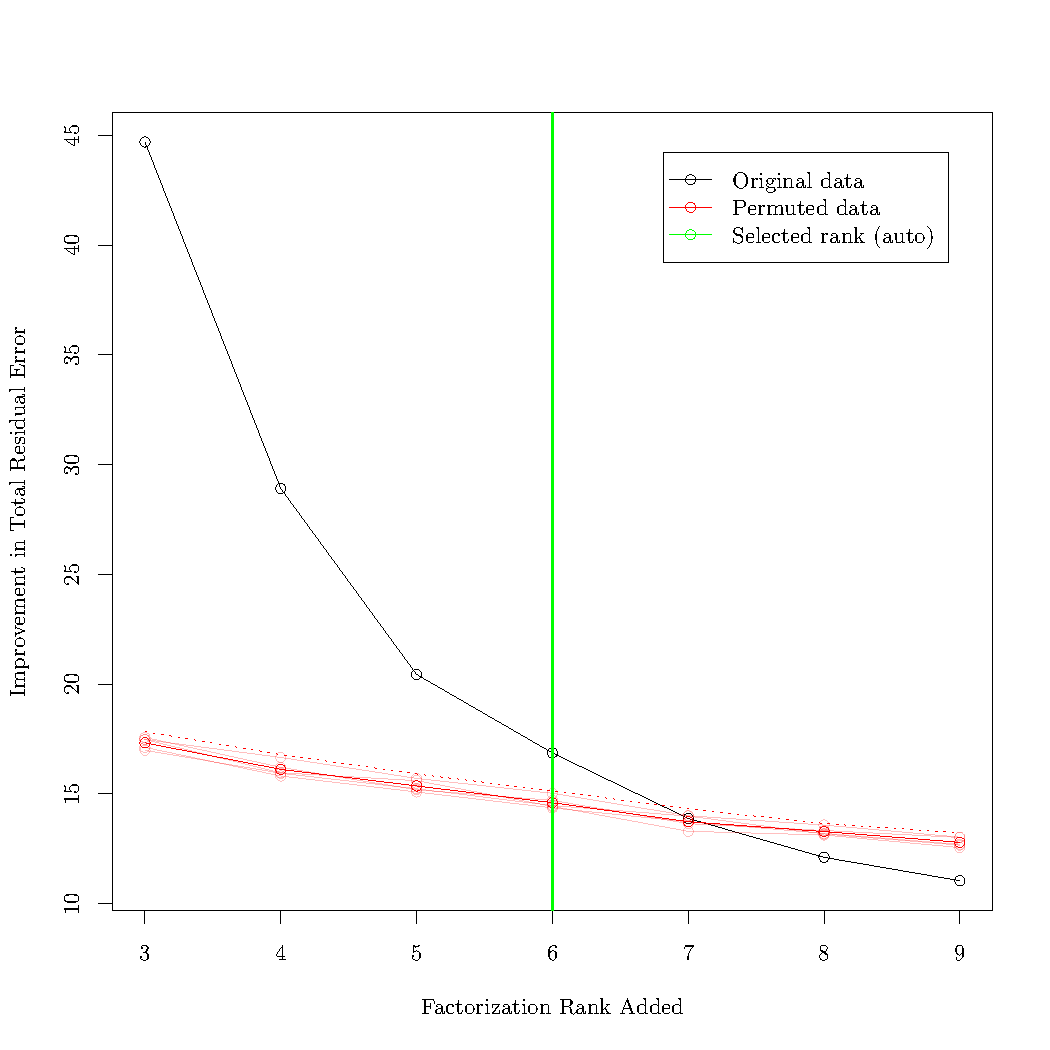
\includegraphics[width=.7\linewidth]{analysis/biosurv/reports/18_SIS_diag_dsd_final/figure/nmf-rank-plots-2}
\caption[Automatic selection of \texorpdfstring{\acrshort{NMF}}{NMF} factorization rank]{Automatic selection of factorization rank.  \acrshort{SNMFL} was performed for varying ranks on either unpermuted data (black line) or data permuted within samples (orange lines), and the improvement in total residual approximation error $\|A - W H\|_F$ calculated.  The highest added rank for which the error improvement on unpermuted data exceeded that of permuted data plus two standard deviations (threshold shown by dotted orange line) was the final selected rank (indicated by a green line).}\label{fig:sigs-nmf-rank}
\end{figure}

\fcardinal{500} random restarts of rank 6 \gls{SNMFL} were then performed on the survival-associated gene matrix to yield the final factorization.  The resultant clustering consensus matrix was stable (\fref{fig:sigs-nmf-consensus}), and the basis matrix $W$ was reasonably sparse (\fref{fig:sigs-nmf-basis}).  Sparsity of the basis matrix is a desirable condition for this analysis, as it indicates that metagenes are largely distinct transcriptional modules, with little overlap in terms of shared transcripts with high loadings; \gls{SNMFL} was selected against alternative \gls{NMF} algorithms as its design favours solutions with sparse $W$.  A table of values of the basis matrix $W$ is available as \Aref{app:sigs-w-matrix} on \pref{app:sigs-w-matrix}.

\begin{figure}[!htbp]
\centering
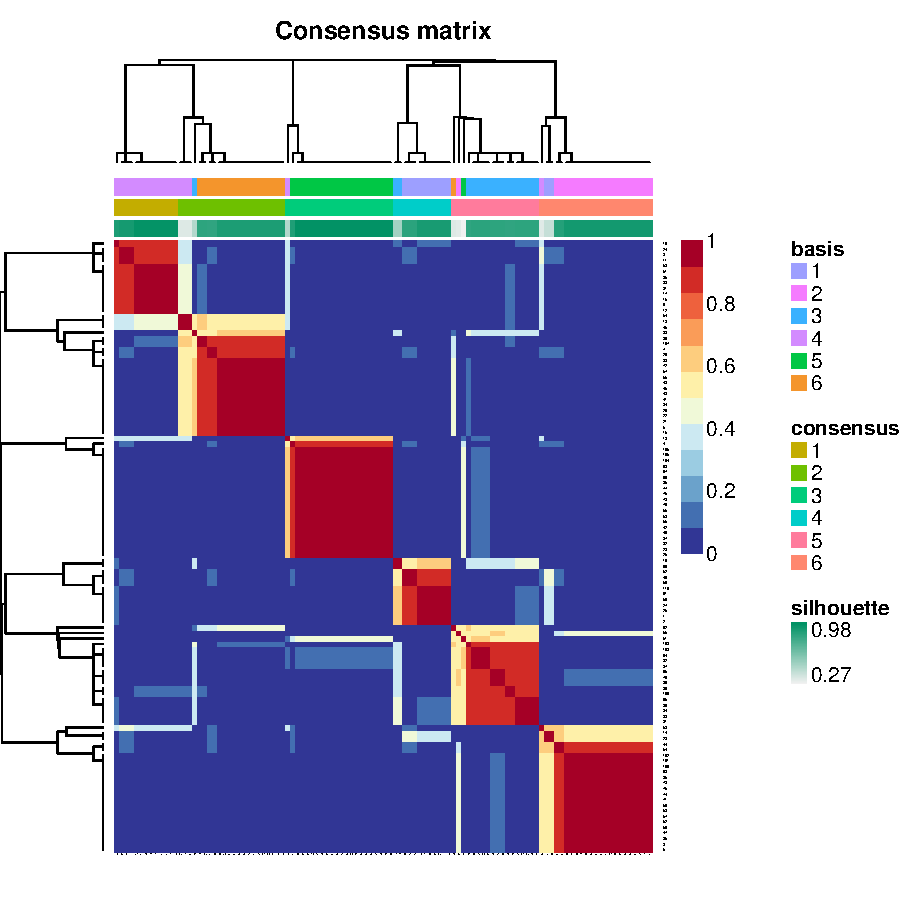
\includegraphics[width=.7\linewidth]{analysis/biosurv/reports/18_SIS_diag_dsd_final/figure/nmf-plots-1}
\caption[Consensus matrix for the final rank-6 clustering]{Clustering consensus matrix for the final rank-6 clustering.  Colours indicate the stability of gene (in rows) and sample (in columns) clusters across random restarts of the factorization; at rank 6 this factorization was largely stable, with identical clusters assigned in all \fcardinal{500} random restarts to the majority of genes and samples.}\label{fig:sigs-nmf-consensus}
\end{figure}

\begin{figure}[!htbp]
\centering
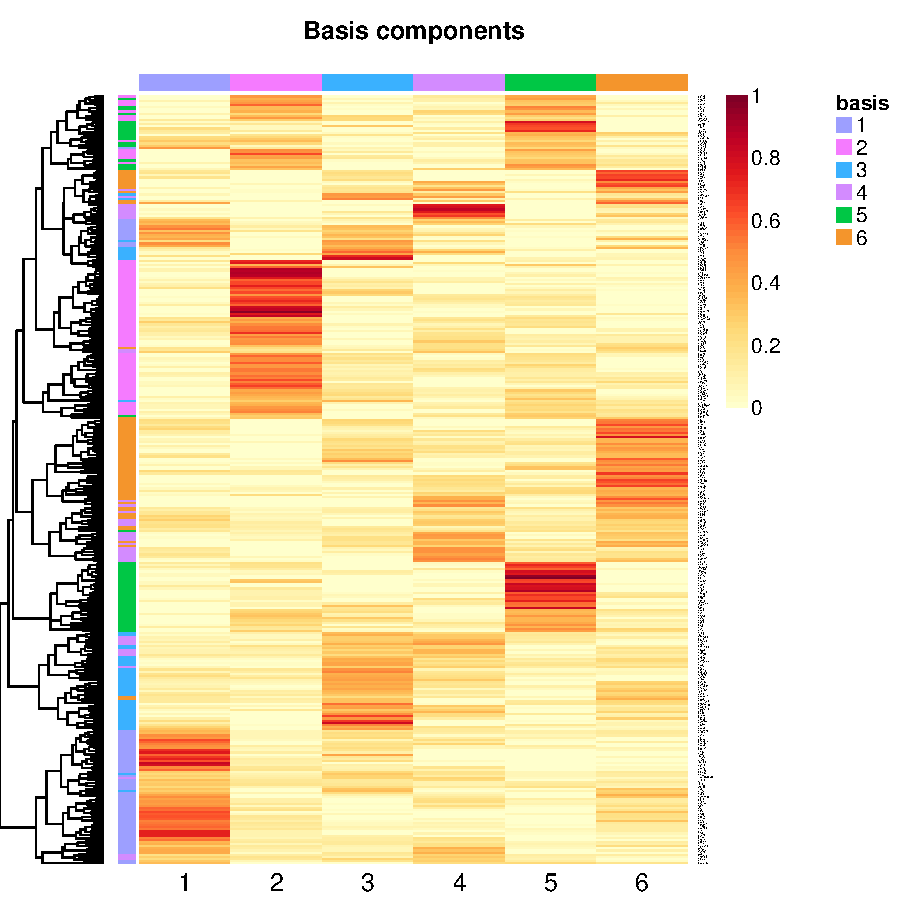
\includegraphics[width=.7\linewidth]{analysis/biosurv/reports/18_SIS_diag_dsd_final/figure/nmf-plots-2}
\caption[Basis matrix \texorpdfstring{$W$}{W} of the final \texorpdfstring{\acrshort{SNMFL}}{SNMF/L} factorization]{Basis matrix $W$ of the final \acrshort{SNMFL} factorization.  Rows represent genes, and columns metagenes, with cell colours proportional to the loading of a given gene on a given metagene.  The loadings are sparse within rows, indicating that the metagenes are modular, each affecting the expression of largely distinct sets of target genes.  A table of values of this basis matrix is available as \Aref{app:sigs-w-matrix} on \pref{app:sigs-w-matrix}.}\label{fig:sigs-nmf-basis}
\end{figure}

\paragraph{Three metagenes together formed a prognostic model}
The transcription patterns of genes associated with survival in the \gls{APGI} cohort could be decomposed into just six largely distinct metagenes.  Due to the presence of false positives in the 361 screened input genes, some of the metagenes will have no strong association with outcome.  To identify which of the six metagenes were ultimately predictive of patient survival, I performed \gls{LASSO} regression on the 110-patient \gls{APGI} discovery cohort data, using \gls{NNLS}-estimated coefficients of each of the six metagenes as marginal predictors of outcome.  The \gls{LASSO} regularization parameter $\lambda$ was chosen by 10-fold cross-validation to be the highest value for which the mean test set partial likelihood deviance was within one standard error of the lowest mean value.  This resulted in a final model in which three metagenes, MG1, MG2, and MG5, were selected as prognostic (\fref{fig:sigs-resub-lasso-track}).

\begin{figure}[!htbp]
\centering
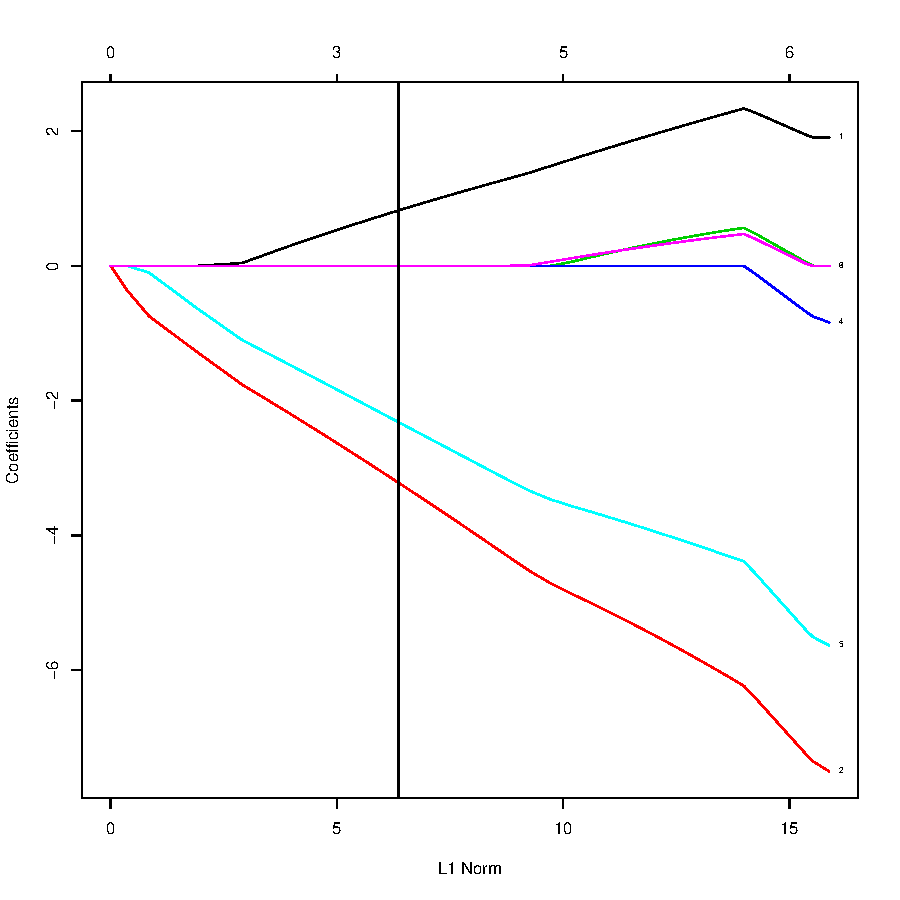
\includegraphics[width=.7\linewidth]{analysis/biosurv/reports/18_SIS_diag_dsd_final/figure/nmf-metagene-glmnet-plots-2}
\caption[Fit trajectory of the \texorpdfstring{\acrshort{LASSO}}{LASSO} predicting \texorpdfstring{\acrshort{DSS}}{DSS} from metagene coefficients]{Coefficient vs penalty fit trajectories for the \acrshort{LASSO} model predicting \gls{DSS} from metagene expression.  Each line represents the model coefficient for a metagene as the model is smoothly varied from a null model (L1 norm = 0), to a full unpenalised Cox fit (L1 norm $\approx$ 16).  The vertical line indicates the optimal value of L1 norm as selected by the 1SE criterion on 10-fold cross-validation; at this point in the trajectory only metagenes MG1, MG2, and MG5 contribute to prognosis estimates.}\label{fig:sigs-resub-lasso-track}
\end{figure}

\paragraph{Prognostic metagenes define two axes of cell transcription}
Further investigation of the three prognostic metagenes revealed that they were associated: \gls{APGI} patient coefficients for pairs MG1 and MG5, and MG2 and MG6 (the latter not selected by the \gls{LASSO}), were mutually exclusive (\fref{fig:sigs-coef-mutualexclusion}, Kendall's $\tau$ test $P < 1 \times 10^{-6}$ for each pair).  This suggested that both metagenes in each pair captured the signal of a single axis of cell behaviour, with one measuring activation of the axis, and the other deactivation.  For subsequent work I therefore combined the signals of the metagenes within each axis, to give axis activity summaries: $\text{Axis A1 activity} = \text{MG1 coefficient} - \text{MG5 coefficient}$; $\text{Axis A2 activity} = \text{MG6 coefficient} - \text{MG2 coefficient}$.  Activation values for axes A1 and A2 were uncorrelated, indicating that these axes were orthogonal processes operating in the \gls{APGI} cohort tumours (\fref{fig:sigs-axis-pairs}, Kendall's $\tau$ test $P = 0.21$).  Metagenes MG3 and MG4 also formed a mutually exclusive pair (not shown), but were not investigated further, as neither was determined to be prognostic by the metagene \gls{LASSO}.

\begin{figure}[!htbp]
\centering
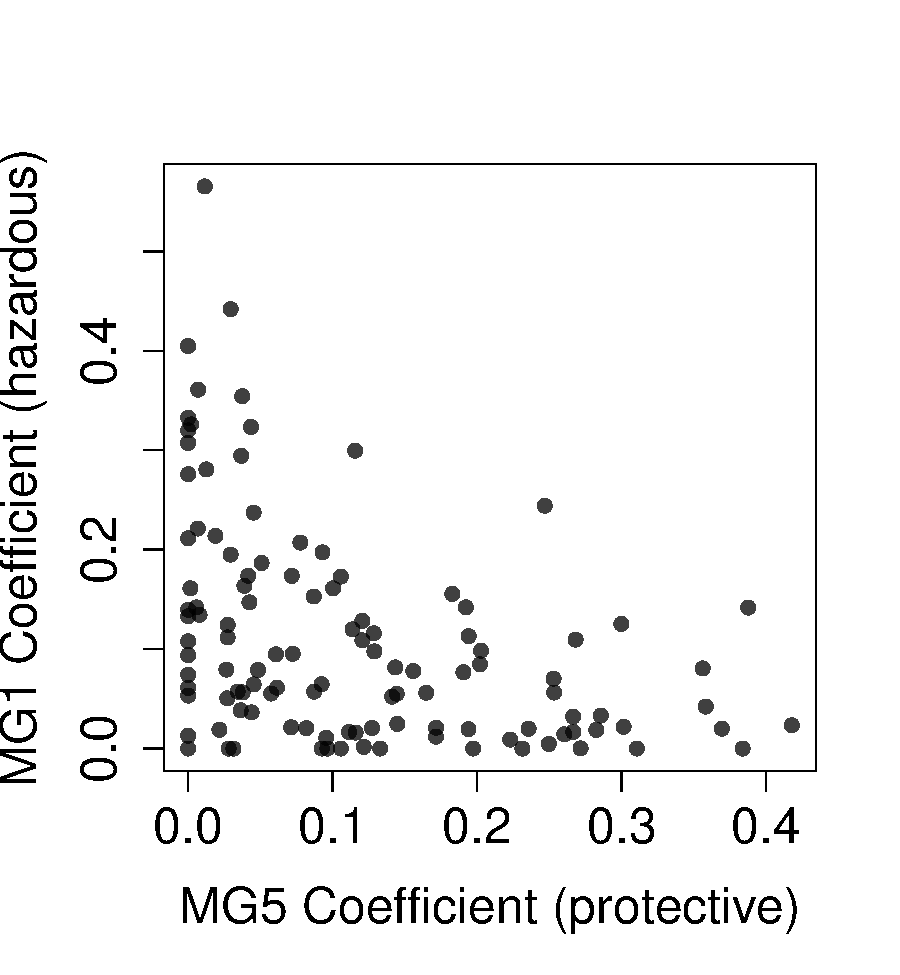
\includegraphics[width=.45\linewidth]{analysis/biosurv/reports/18_SIS_diag_dsd_final/figure/metagene-pairs-8}
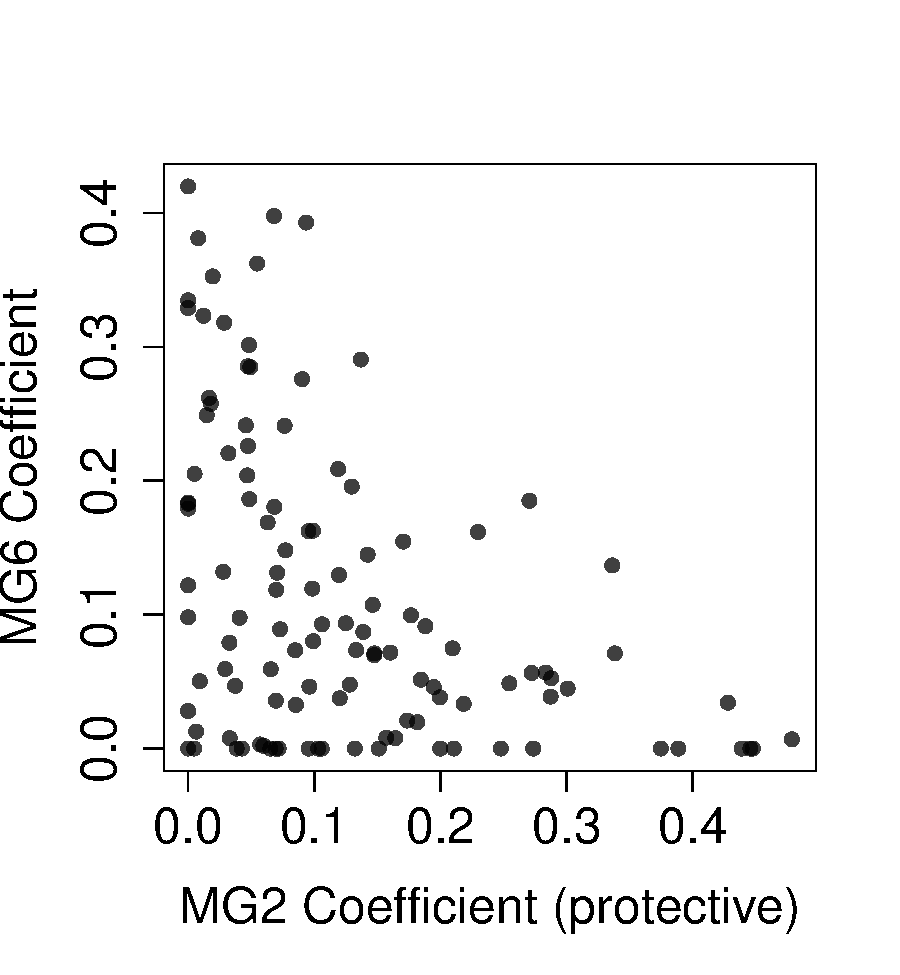
\includegraphics[width=.45\linewidth]{analysis/biosurv/reports/18_SIS_diag_dsd_final/figure/metagene-pairs-9}
\caption[Prognostic metagenes form two axes of cell state]{Prognostic metagenes form two axes of cell state.  Metagene pairs MG1 and MG5, and MG2 and MG6, displayed mutually exclusive coefficient patterns in the \acrshort{APGI} cohort, and could be combined to form just two axes of cell state.}\label{fig:sigs-coef-mutualexclusion}
\end{figure}

\begin{figure}[!htbp]
\centering
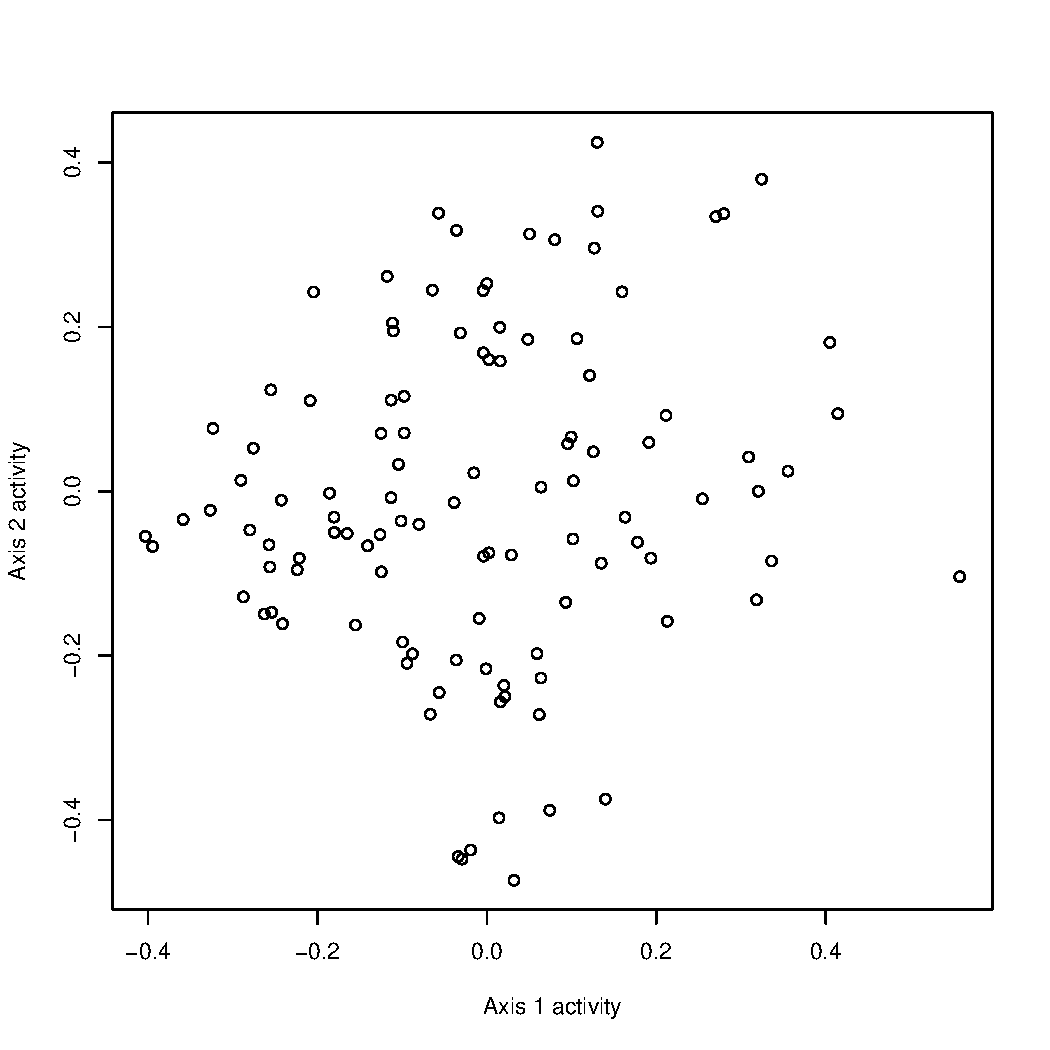
\includegraphics[width=.7\linewidth]{analysis/biosurv/reports/18_SIS_diag_dsd_final/figure/metagene-pairs-10}
\caption[Prognostic axes are uncorrelated]{Prognostic axis signals are uncorrelated.  Activity estimates of axes defined by highly correlated mutually exclusive metagene pairs (Axis A1 = MG1 - MG5, axis A2 = MG6 - MG2) were uncorrelated (Kendall $\tau$ test $P = 0.21$), indicating that these axis signals encoded orthogonal outcome-associated processes within tumours.}\label{fig:sigs-axis-pairs}
\end{figure}

\paragraph{The \texorpdfstring{\acrshort{PARSE}}{PARSE} score}
A repeat of the previous \gls{LASSO} fit with 10-fold \gls{CV}, this time using predictors of A1 activity, A2 activity, and the A1:A2 interaction, identified both A1 and A2, but not their interaction, as useful predictors of outcome.  Coefficients from the \gls{LASSO} fit were used to define a new risk score, the \gls{PARSE}, as $\text{PARSE score} = 1.354 \times \text{A1 activity} + 1.548 \times \text{A2 activity}$.

Exact calculation of the \gls{PARSE} score requires the solution of a number of \gls{NNLS} problems, which presents a potential barrier to use.  An approximation to \gls{PARSE} can be derived by relaxing the non-negative constraint; this approximation requires only a weighted mean of gene expression estimates, and is detailed in \Aref{app:sigs-parse-approx} on \pref{app:sigs-parse-approx}.

\paragraph{Validation of the \texorpdfstring{\acrshort{PARSE}}{PARSE} score}
External validation confirmed that the \gls{PARSE} score was prognostic in other cohorts, including in cancers other than \gls{PDAC}.  \Gls{PARSE} score was significantly prognostic in \gls{PDAC} cohorts GSE28735~\cite{Zhang2013} (LRT $P = 0.0149$) and \gls{TCGA} paad (LRT $P = 0.0156$), but not in GSE21501~\cite{Stratford2010} (LRT $P = 0.115$).  When assessed against all \gls{TCGA} cancers for which at least 50 patients had both an event and complete RNASeq data, the \gls{PARSE} score was also significantly prognostic for head and neck squamous cell carcinoma, kidney renal clear cell carcinoma, lower grade glioma, and lung adenocarcinoma, at a 5\% \gls{FWER} (\tref{tab:sigs-validation-tcga}, column a).  This significant result reflected the ability of the \gls{PARSE} score to stratify patients into risk groups in a range of solid tumours, as illustrated in \fref{fig:sigs-km}.

Meta-PCNA is a 130-gene signature of cell proliferation that has been found to be generally prognostic in a number of cancer cohorts~\cite{Venet2011}.  To exclude the possibility that \gls{PARSE} score simply recapitulated the known meta-PCNA signature, I examined whether \gls{PARSE} contributed additional prognostic information to meta-PCNA in the large \gls{TCGA} cohorts.  In \gls{TCGA} kidney renal clear cell carcinoma, lower grade glioma, and lung adenocarcinoma, there was significant evidence that the \gls{PARSE} score provided prognostic information beyond that given by meta-PCNA, at a 5\% \gls{FWER} (\tref{tab:sigs-validation-tcga}, column b).

\begin{table}[!htbp]
\centering
\caption[\texorpdfstring{\acrshort{PARSE}}{PARSE} score is prognostic in a range of \texorpdfstring{\acrshort{TCGA}}{TCGA} cancers]{The \acrshort{PARSE} score is prognostic in a range of \acrshort{TCGA} cancers.  P-values are from likelihood ratio tests either comparing a Cox model with \acrshort{PARSE} score as a linear predictor, to a null model (a); or a Cox model with \acrshort{PARSE} and meta-PCNA scores as linear predictors, against one with meta-PCNA alone (b).  Shaded cells are significant at a 5\% \acrshort{FWER} following Holm's correction.  \acrshort{TCGA} study codes: \emph{glm}: glioblastoma multiforme; \emph{hnsc}: head and neck squamous cell carcinoma; \emph{kirc}: clear cell kidney carcinoma; \emph{lgg}: lower grade glioma; \emph{luad}: lung adenocarcinoma; \emph{lusc}: lung squamous cell carcinoma; \emph{ov}: ovarian serous cystadenocarcinoma.}\label{tab:sigs-validation-tcga}
\resizebox{\textwidth}{!}{
\begin{tabular}{@{}lllll@{}}
\toprule
TCGA   & Number of & Number of & Risk score  & Improvement \\
study  & events    & patients  & P-value (a) & P-value (b) \\ \midrule
gbm    & 54   & 143    & 0.2287                           & 0.1587                           \\
hnsc   & 124  & 367    & \cellcolor[HTML]{C0C0C0}$8.08 \times 10^{-3}$  & 0.0108                           \\
kirc   & 153  & 497    & \cellcolor[HTML]{C0C0C0}$2.03 \times 10^{-12}$ & \cellcolor[HTML]{C0C0C0}$2.89 \times 10^{-3}$  \\
lgg    & 53   & 272    & \cellcolor[HTML]{C0C0C0}$1.49 \times 10^{-5}$  & \cellcolor[HTML]{C0C0C0}$7.85 \times 10^{-3}$  \\
luad   & 106  & 431    & \cellcolor[HTML]{C0C0C0}$8.34 \times 10^{-6}$  & \cellcolor[HTML]{C0C0C0}$1.04 \times 10^{-4}$  \\
lusc   & 117  & 395    & 0.9624                           & 0.4110                           \\
ov     & 115  & 251    & 0.0238                           & 0.0178                           \\ \bottomrule
\end{tabular}
}
\end{table}

\clearpage
\begin{figure}[!htbp]
  \centering

  \subbottom[\texorpdfstring{\acrshort{APGI}}{APGI} cohort (Resubstituted)]{
    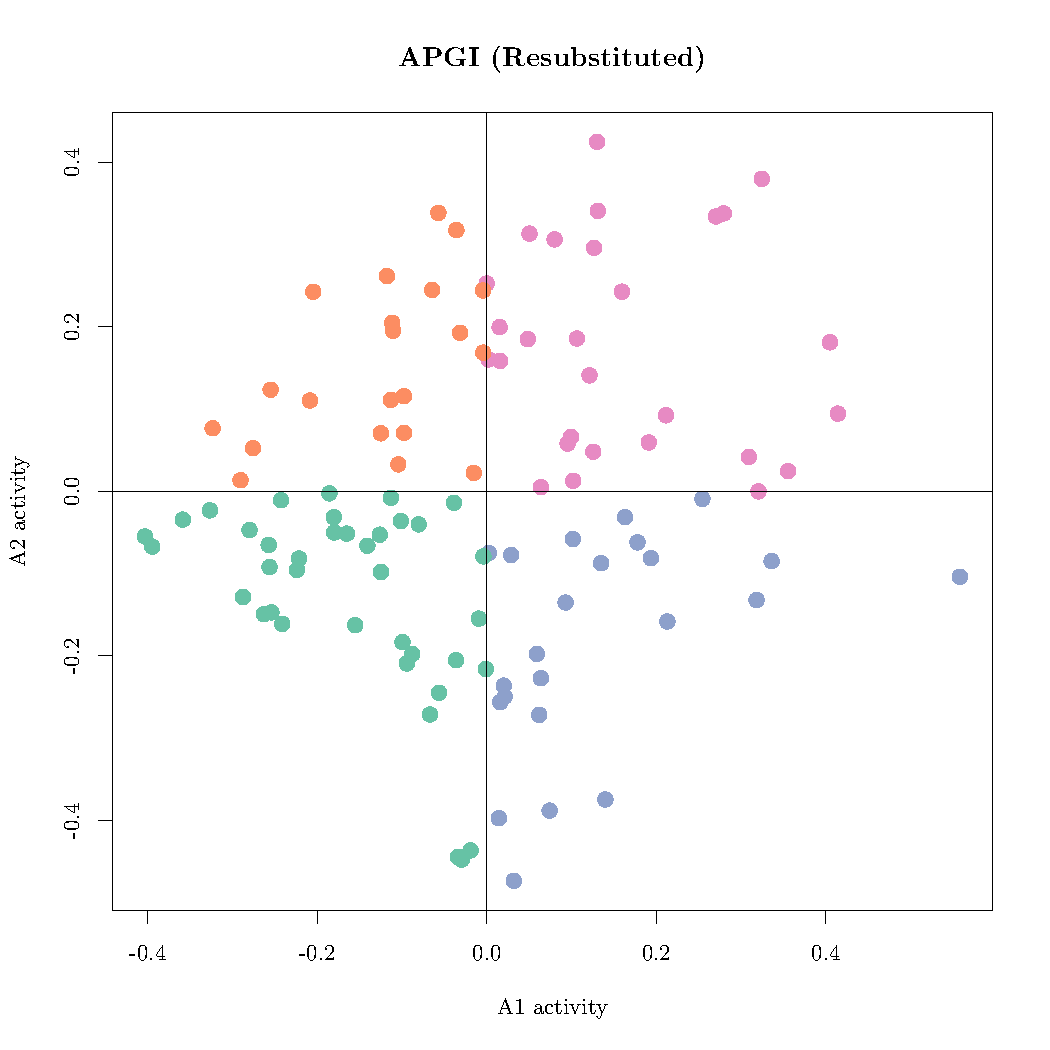
\includegraphics[width=.5\textwidth]{analysis/biosurv/reports/18_SIS_diag_dsd_final/figure/km-curves-1}
    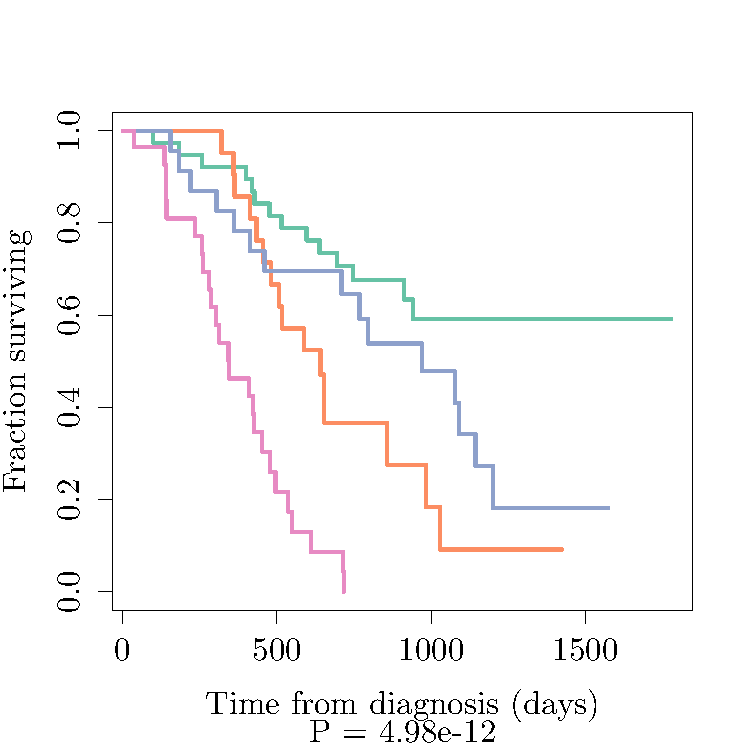
\includegraphics[width=.5\textwidth]{analysis/biosurv/reports/18_SIS_diag_dsd_final/figure/km-curves-2}
    \label{figs:sigs-km-apgi}}

  \subbottom[\texorpdfstring{\acrshort{TCGA}}{TCGA} kirc cohort]{
    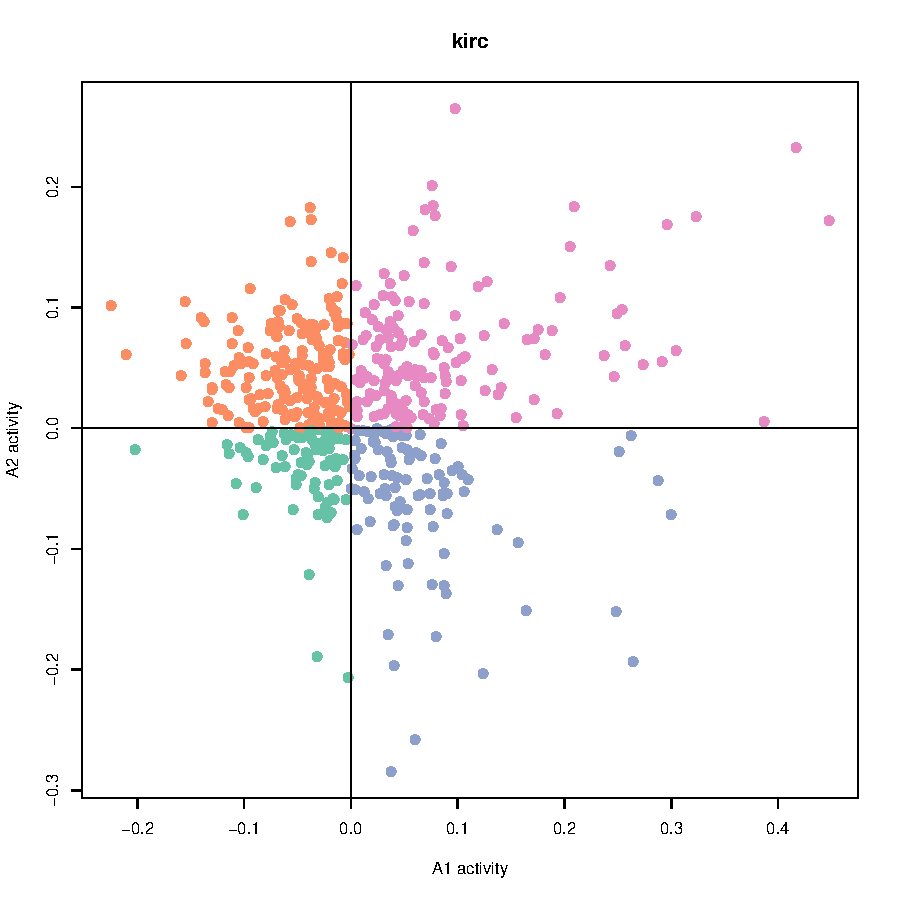
\includegraphics[width=.5\textwidth]{analysis/biosurv/reports/18_SIS_diag_dsd_final/figure/km-curves-9}
    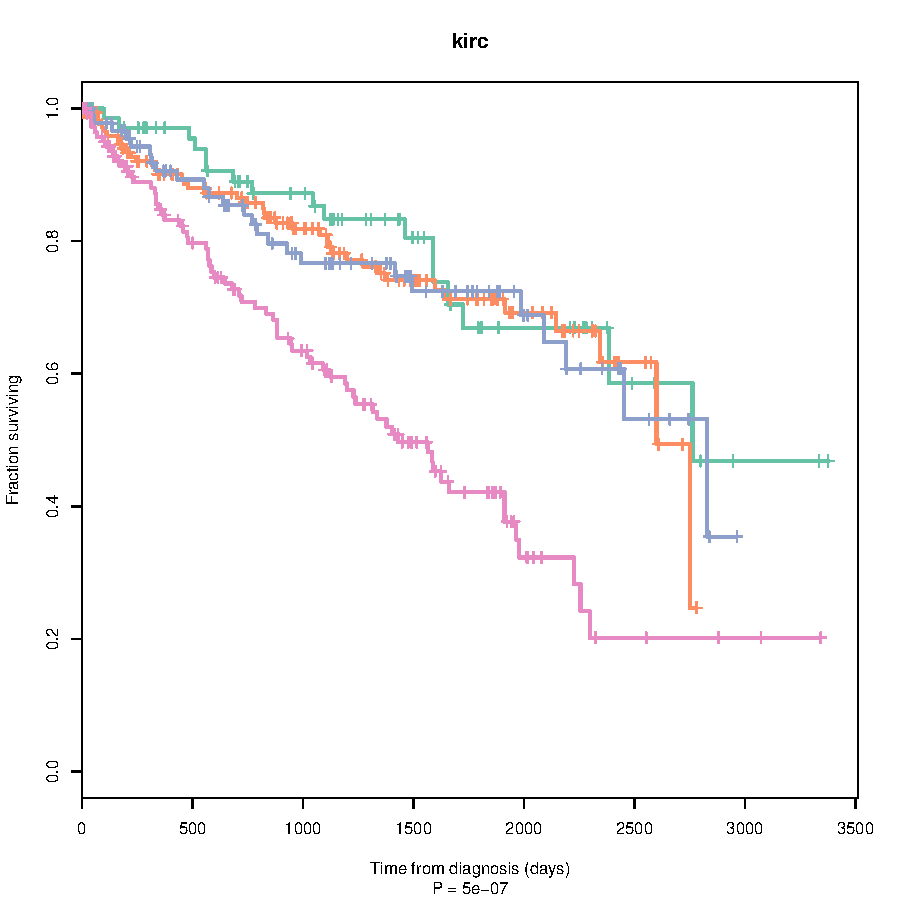
\includegraphics[width=.5\textwidth]{analysis/biosurv/reports/18_SIS_diag_dsd_final/figure/km-curves-10}
    \label{figs:sigs-km-kirc}}
  \caption[Survival subgroups defined by \texorpdfstring{\acrshort{PARSE}}{PARSE} score axes in different tumours]{\acrshort{PARSE} score axes define patient subgroups with differing outcome in a range of solid tumours.  Activities for axes A1 and A2 of the \acrshort{PARSE} score were calculated on the labelled cohorts, and patients split into four subgroups based on the sign of A1 and A2 activities (left panels).  The four subgroups thus defined displayed significantly differing clinical courses (right panels).  (continued...)}\label{fig:sigs-km}
\end{figure}

\begin{figure}[!htbp]
  \centering

  \contsubbottom[\texorpdfstring{\acrshort{TCGA}}{TCGA} lgg cohort]{
    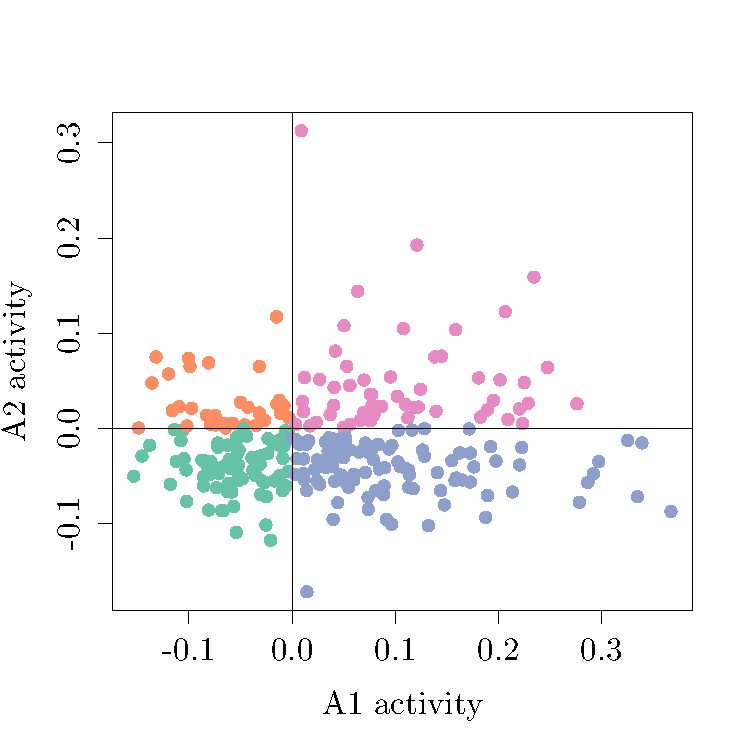
\includegraphics[width=.5\textwidth]{analysis/biosurv/reports/18_SIS_diag_dsd_final/figure/km-curves-11}
    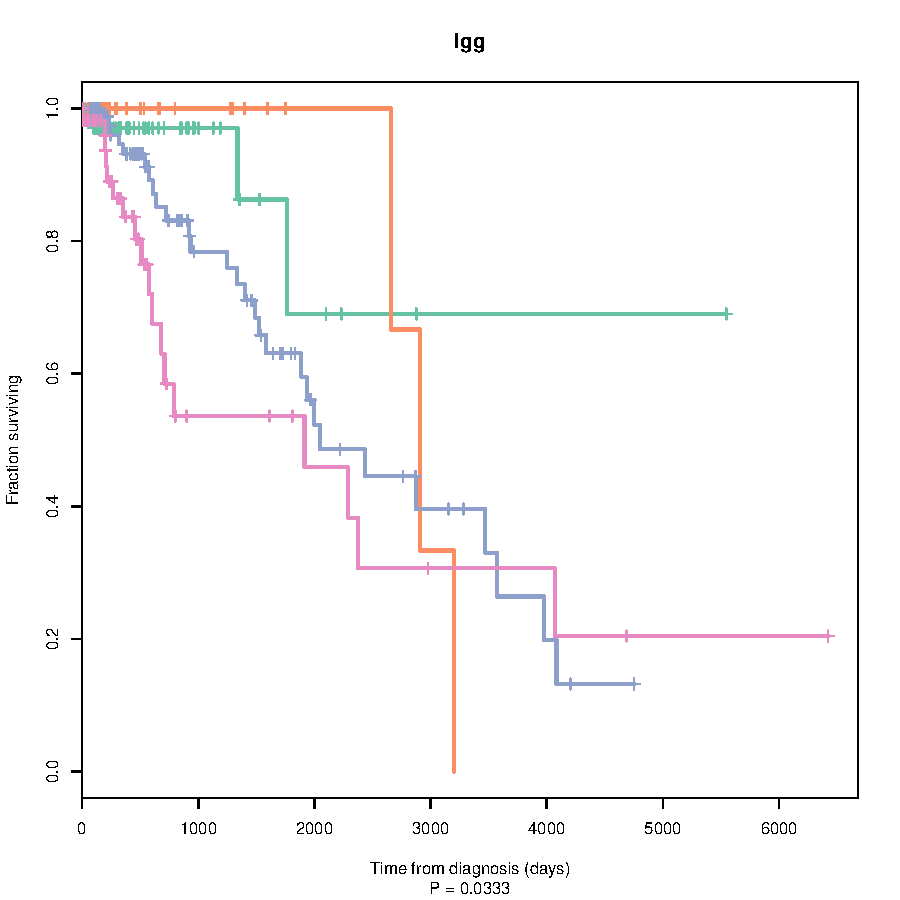
\includegraphics[width=.5\textwidth]{analysis/biosurv/reports/18_SIS_diag_dsd_final/figure/km-curves-12}
    \label{figs:sigs-km-lgg}}

  \contsubbottom[\texorpdfstring{\acrshort{TCGA}}{TCGA} luad cohort]{
    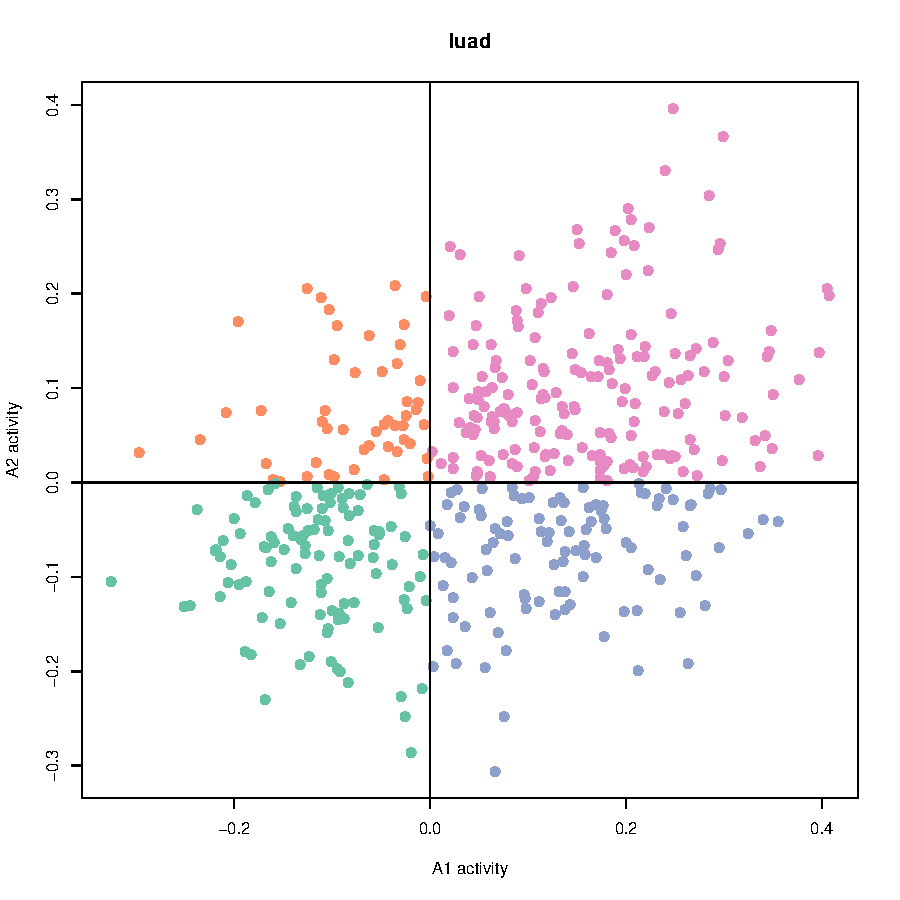
\includegraphics[width=.5\textwidth]{analysis/biosurv/reports/18_SIS_diag_dsd_final/figure/km-curves-13}
    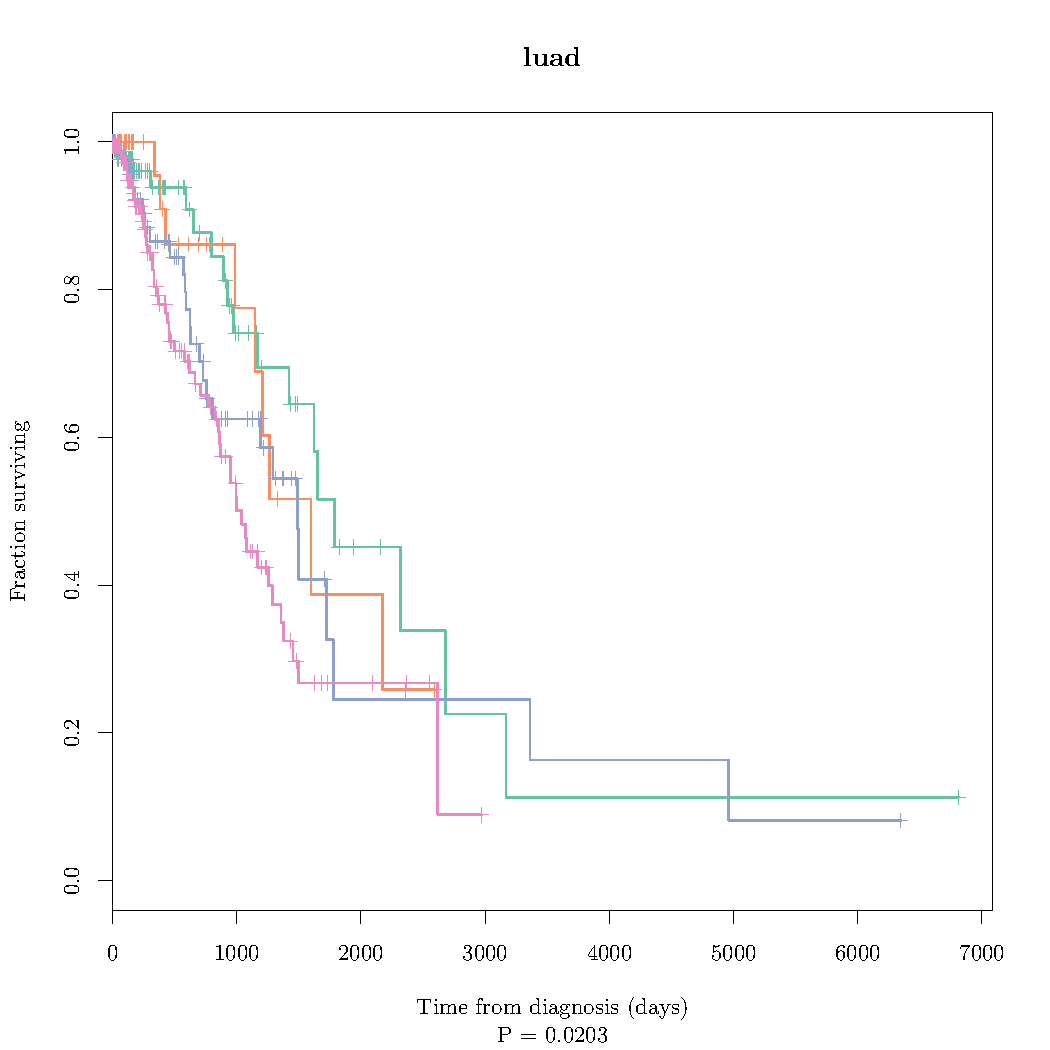
\includegraphics[width=.5\textwidth]{analysis/biosurv/reports/18_SIS_diag_dsd_final/figure/km-curves-14}
    \label{figs:sigs-km-luad}}
    
  \contcaption{(Concluded). \acrshort{PARSE} score axes define patient subgroups with differing outcome in a range of solid tumours.  Activities for axes A1 and A2 of the \acrshort{PARSE} score were calculated on the labelled cohorts, and patients split into four subgroups based on the sign of A1 and A2 activities (left panels).  The four subgroups thus defined displayed significantly differing clinical courses (right panels).}
\end{figure}


\subsection{\texorpdfstring{\acrshort{PARSE}}{PARSE} identifies proliferation and \texorpdfstring{\acrshort{EMT}}{EMT} as fundamental processes controlling survival in \texorpdfstring{\acrshort{PDAC}}{PDAC}}
To link the two prognostic axes that form the \gls{PARSE} score with potential underlying biology, axis activities on the \gls{APGI} discovery cohort were compared to clinical variates, known survival signatures, and scores for signatures from the \gls{MSIGDB}~\cite{Subramanian2005}.

\paragraph{Axis A1}
\gls{PARSE} axis A1 score (MG1 $-$ MG5) was significant positively correlated with estimates of cancer cell fraction in the tumour as assessed by qPure~\cite{Song2012} \footnote{qPure is a tool to determine cancer cell fraction in a mixed tumour DNA sample by quantification of \gls{BAF} separation from \gls{SNP} genotyping array data.  I contributed to the development of qPure, by proposing and designing the experiments that ultimately led to the creation of the tool, and by designing the final calibration model that links \gls{BAF} separation to cancer DNA fraction.} (Kendall's $\tau = 0.284$, $n = 110$, \tref{tab:sigs-mg-cpvs}), although the strength of this association was marginal (linear model $R^2 = 0.155$).  No other \glspl{CPV} were significantly associated with A1 score after correction for multiple testing (\tref{tab:sigs-mg-cpvs}).

\gls{MSIGDB} correlations, as well as comparisons to a general proliferative signature, revealed that A1 primarily reflected the proliferative state of cells.  A1 signal was very strongly correlated with meta-PCNA~\cite{Venet2011} score (Kendall's $\tau = 0.663$, $n = 110$, \fref{fig:sigs-axis1-pcna}), a relationship supported by its close association to cell cycle-related \gls{MSIGDB} signatures (\Aref{app:sigs-msigdb-corrs-axis1} on \pref{app:sigs-msigdb-corrs-axis1}).

\paragraph{Axis A2}
Among the clinical variables tested, \gls{PARSE} axis A2 (MG6 $-$ MG2) was negatively correlated with qPure tumour cell fraction, and positively associated with higher tumour histological grade (\tref{tab:sigs-mg-cpvs}).  The negative association between A2 score and tumour cell fraction is the opposite of the positive association seen with A1 score, despite high levels of both A1 and A2 being associated with poor prognosis.  This reveals a potential context dependency in the influence of stromal content on survival, where high stromal content of a tumour may indicate either good or poor prognosis, depending on which underlying axis is responsible.  Reflecting the poor prognosis associated with high A2, A2 score was also significantly but weakly dependent on grade: on average, A2 signal was $0.1103$ higher in grade 3 or 4 tumours over grade 1 or 2, with $R^2 = 0.119$.

A number of \gls{MSIGDB} signatures were associated with A2 signals, among them integrins, \gls{ECM} processes, and a signature for LEF1-mediated \gls{EMT} (\Aref{app:sigs-msigdb-corrs-axis2} on \pref{app:sigs-msigdb-corrs-axis2}).  Prompted by the strong positive correlation between A2 and the LEF1 overexpression signature, I investigated the association between A2 signal and score for a general signature of \gls{EMT}, meta-EMT~\cite{Groger2012}.  meta-EMT and A2 signals were strongly positively correlated (Kendall's $\tau = 0.568$, $n = 110$, linear model $R^2 = 0.557$, \ref{fig:sigs-axis2-emt}), even when cancer cell fraction was taken into account (LRT $P = 9.4 \times 10^{-14}$), strongly indicating that A2 signal predominantly encodes \gls{EMT} activity.  A potential link between A2 and inflammation may also be present: A2 signal was strongly positively correlated with the \gls{GSVA} score for \gls{MSIGDB} GNF2\_PTX3 (Kendall's $\tau = 0.593$, \Aref{app:sigs-msigdb-corrs-axis2} on \pref{app:sigs-msigdb-corrs-axis2}), a proxy for expression of the acute phase response protein pentraxin 3.

\paragraph{Link to S100 prognostic biomarkers}
\Cref{chap:nomogram} uses the tissue levels of proteins S100A2 and S100A4 to predict survival with resected \gls{PDAC}.  S100A2 and S100A4 are both considered to be biomarkers of metastasis~\cite{Biankin2009, Lee2014, Tsukamoto2013}, and so we expect their expression to be associated with the putative metastasis-related axis A2.  Although neither S100A2 nor S100A4 were among the set of \fcardinal{361} survival-associated genes, their mRNA abundance estimates were significantly positively correlated with axis A2 signal, with Kendall's $\tau = 0.30$ ($P = 3.25 \times 10^{-6}$) for S100A2, and $\tau = 0.29$ ($P = 5.67 \times 10^{-6}$) for S100A4.

\begin{figure}[!htbp]
\centering
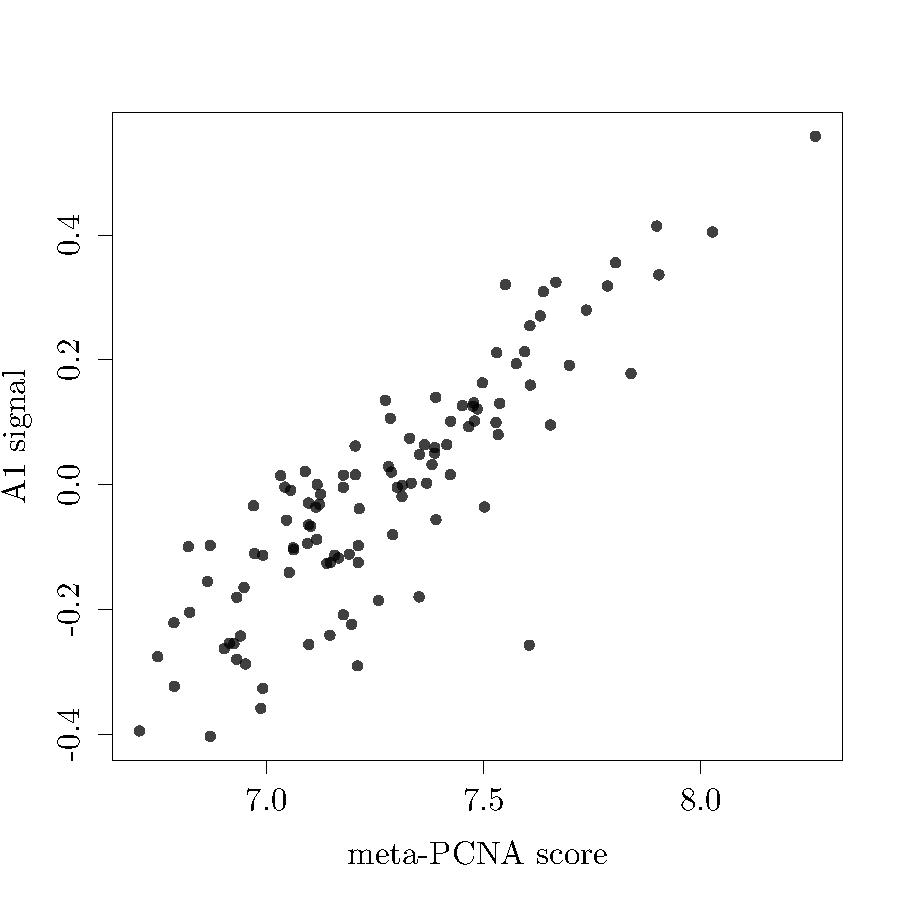
\includegraphics[width=.7\linewidth]{analysis/biosurv/reports/18_SIS_diag_dsd_final/figure/nmf-msigdb-cor-plots-5}
\caption[A1 signal is closely associated with meta-PCNA score]{Axis A1 signal is closely associated with the meta-PCNA signature.  A1 signal and meta-PCNA~\cite{Venet2011} scores were as evaluated on the \acrshort{APGI} training set; Kendall's $\tau = 0.663$, $n = 110$, linear model $R^2 = 0.740$.}\label{fig:sigs-axis1-pcna}
\end{figure}

\begin{table}
\centering
\caption[Association P-values between metagenes and \texorpdfstring{\acrshortpl{CPV}}{CPVs}]{Association P-values between metagenes and \acrshortpl{CPV}.  P-values were either from Kendall $\tau$ tests, in the case of continuous or large ordinate clinical variates, or from ANOVA, in the case of categorical variates.  Only three associations were signficant at a 5\% FWER level by Holm's correction; these are highlighted.  For pathological grade and cancer cell fraction variables, the direction of association is indicated by ($+$) or ($-$) annotations.}\label{tab:sigs-mg-cpvs}
\begin{tabular}{@{}lll@{}}
Variable                   & Axis 1                        & Axis 2                        \\ \midrule
Age at diagnosis           & 0.925                         & 0.666                         \\
Ethnicity                  & 0.771                         & 0.113                         \\
Gender                     & 0.158                         & 0.010                         \\
Histological subtype       & 0.697                         & 0.157                         \\
Invasion                   &                               &                               \\
\quad Perineural           & 0.095                         & 0.225                         \\
\quad Vascular             & 0.650                         & 0.071                         \\
Pack years smoked          & 0.356                         & 0.275                         \\
Pathological grade         & 2.39$\times 10^{-3}$ ($+$)          & \cellcolor[HTML]{C0C0C0}1.30$\times 10^{-4}$ ($+$) \\
Cancer cell fraction       & \cellcolor[HTML]{C0C0C0}2.13$\times 10^{-4}$ ($+$) & \cellcolor[HTML]{C0C0C0}4.11$\times 10^{-4}$ ($-$) \\
Recurrence site            &                               &                               \\
\quad Bone                 & 0.789                         & 0.413                         \\
\quad Brain                & 0.430                         & 0.062                         \\
\quad Liver                & 0.160                         & 0.105                         \\
\quad Lung                 & 0.390                         & 0.713                         \\
\quad Lymph nodes          & 0.933                         & 0.870                         \\
\quad Mesentery            & 0.933                         & 0.121                         \\
\quad Omentum              & 0.139                         & 0.082                         \\
\quad Other                & 0.193                         & 0.161                         \\
\quad Pancreatic bed       & 0.887                         & 0.530                         \\
\quad Pancreas remnant     & 0.534                         & 0.184                         \\
\quad Peritoneum           & 0.916                         & 0.015                         \\
Staging: M                 & 0.441                         & 0.425                         \\
Staging: N                 & 0.252                         & 0.263                         \\
Staging: T                 & 0.264                         & 0.427                         \\
Staging: Overall stage     & 0.061                         & 0.236                         \\
Tumour location            & 0.177                         & 0.139                         \\
Tumour longest axis length & 0.844                         & 0.171                         \\ \bottomrule
\end{tabular}
\end{table}

\begin{figure}[!htbp]
\centering
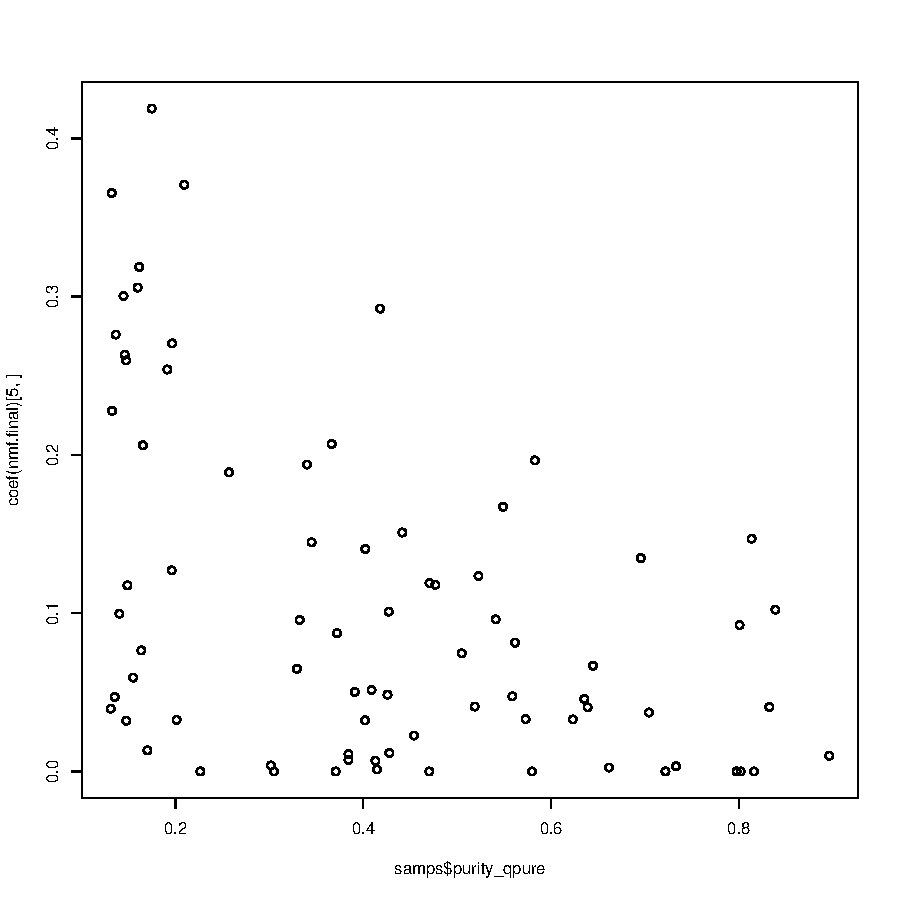
\includegraphics[width=.7\linewidth]{analysis/biosurv/reports/18_SIS_diag_dsd_final/figure/nmf-msigdb-cor-plots-8}
\caption[A2 signal is closely associated with meta-EMT score]{Axis A2 signal is closely associated with a signature of the \gls{EMT}.  A2 signal and meta-EMT~\cite{Groger2012} scores were as evaluated on the \acrshort{APGI} training set; Kendall's $\tau = 0.568$, $n = 110$, linear model $R^2 = 0.557$.}\label{fig:sigs-axis2-emt}
\end{figure}

\section{Discussion}
At the molecular level, the phenomenon of cancer has long been recognised as a composite of many processes~\cite{Hanahan2011}, however the relative importance of each process to a particular type of cancer has been largely uncertain.  In pancreas cancer, a huge number of individual biomarkers are known~\cite{Harsha2009}, and attempts have been made to stratify cancers into empirical molecular subtypes~\cite{Collisson2011}, but no studies have yet provided a comprehensive analysis of which basic hallmarks of cancer are actually important in determining patient outcome.  This chapter fills that gap in knowledge, by exhaustively identifying proliferation and the \gls{EMT} as the major molecular processes that control survival of patients with pancreas cancer.

%The thesis underlying this work was that fundamental disease processes control the survival of patients with resected \gls{PDAC}, and that these processes can be identified from patterns of gene expression in patient tumours.  To test this thesis, a global biology-agnostic approach was used to exhaustively identify expression modules strongly associated with outcome, and these modules were then linked to biological processes.  Two independent outcome-associated modules were identified, and comparisons with published gene signatures indicated that one of these modules was likely measuring proliferative activity, and the other the \gls{EMT}, in the tumours.

Cancer is fundamentally a proliferative process: it is through inappropriate and continued proliferation, and the consequent destruction of normal tissues and disruption of homeostasis, that cancer progressively overwhelms the body.  The prognostic axis A1 discovered here was strongly correlated with the meta-PCNA signature of cell proliferation~\cite{Venet2011} (\fref{fig:sigs-axis1-pcna}), and appears to encode overall proliferative activity in patient tumours.  The association between axis A1 activity and outcome was not unique to pancreas cancer: A1 was prognostic in a number of solid tumours, suggesting that proliferative activity is a prognostic marker of wider applicability than originally reported.  Interestingly, there is evidence that the effect of proliferative level on outcome can be conditional on other biology: in the \gls{TCGA} clear cell kidney cohort, high A1 activity was only associated with poorer outcome when axis A2 activity was also high.

Signals of the A2 axis were well-correlated with the meta-EMT signature~\cite{Groger2012} (\fref{fig:sigs-axis2-emt}), suggesting that A2 levels reflected the activity of \gls{EMT} processes within tumours.  The \gls{EMT} is a major enabling step in metastasis, the process by which most cancers are ultimately lethal~\cite{Talmadge2010}.  The \gls{EMT} has a particular importance to pancreas cancer, as it is believed that occult metastases, present at the time of primary tumour resection, are the major cause of recurrence in resected patients (see \Cref{chap:nomogram} for detailed discussion of this point).  A2 signal, and by proxy \gls{EMT} activity, may be acting as a marker of tumour metastatic ability, and indirectly reflect the likelihood that a patient will have metastatic disease at the time of resection.  This possibility is supported by the positive correlation between axis A2 signal, and levels of mRNA for S100A2 and S100A4, which are suspected biomarkers of occult metastasis in \gls{PDAC}.  In the presence of such metastases, the effectiveness of primary resection is greatly reduced, and earlier death of the patient is to be expected.  The observed worsening prognosis with increasing A2 signal in postoperative patients is consistent with this proposed mechanism, and suggests that A2 loadings could be adapted to identify markers of early metastasis to aid clinical decision making.

Proliferation and the \gls{EMT} are two of the ten major hallmarks of cancer~\cite{Hanahan2011}, and so it is unsurprising that they are so closely associated with patient survival.  What \emph{is} surprising is that the majority of hallmarks do \emph{not} appear to be strongly associated with outcome in resected \gls{PDAC}.  In particular, the absence of stromal or inflammatory signatures is unexpected given that \gls{PDAC} cells are almost always surrounded by extensive stroma, which is believed to be a clinically significant component of the disease~\cite{Luo2012}.

Transcription patterns linked to the tumour stroma may form a prognostic module that was missed by this work.  Desmoplastic stroma is a pervasive and significant component of \gls{PDAC} tumours~\cite{Hidalgo2010}, but its relevance to outcome is unclear: high tumour stromal content has been reported to be both harmful~\cite{Luo2012, Provenzano2012}, and protective~\cite{Rhim2014, Sinn2014}; and the association between stroma activity and outcome is similarly ambiguous~\cite{Bever2014, Sinn2014}.  This divergence in experimental findings suggests that the effect of the stroma on outcome is modulated by uncontrolled confounding factors.  In such a situation, the approach taken in this work can not reliably identify stroma-associated transcriptional modules, even if these modules are genuinely linked to outcome.  Some evidence that this may have occurred is given by the inverse association between tumour stroma content, as measured by $1 - \mathrm{qPure score}$, and axis A1 and A2 signals (\tref{tab:sigs-mg-cpvs}).  This work's potential poor sensitivity in the presence of confounding factors is not restricted to the discovery of stromal effects, but is a general consequence of the marginal variable screening approach that was used.

The signature discovery approach undertaken in this work was tuned to detect all major transcriptional modules affecting outcome in pancreas cancer, but may have missed less significant modules that have a minor influence on survival, only affect a relatively small subset of patients, or are masked by interaction effects.  The nature of the modules detected by the selection-factorization approach used here is strongly dependent on the performance of the initial hard-thresholding prognostic gene selection step.  This work used a simple marginal screening approach that enjoys performance guarantees for near-orthogonal designs~\cite{Fan2008}, but may be unreliable for the highly correlated measurements seen in gene expression data.  In particular, genes with high conditional, but low marginal, associations with survival; or effects on outcome that are weak, or restricted to a small subgroup of patients; may have been missed by the initial screen.  Any minor modules encoded by the expression of these missed genes would not have been identified by this work.  Despite its potential insensitivity, simple marginal screening was the only practical method for prognostic gene identification in the \gls{APGI} training cohort, and still succeeded in defining the two major signatures that reflect outcome in resected pancreas cancer.  Future analyses on larger cohorts may be able to identify additional minor prognostic modules, such as potential stroma-associated modules, by adjusting for the signals of axes A1 and A2 identified in this work.

The \gls{PARSE} prognostic score, and its axis A1 and A2 components, were prognostic in a range of validation cohorts, both of \gls{PDAC}, and in other solid tumours.  This latter result was surprising, and suggests the importance of proliferation and the \gls{EMT} as determinants of differential prognosis in a range of malignancies.  The precise nature of association was dependent on cohort: in \gls{PDAC} and \gls{TCGA} lung cancer, A1 and A2 signals contributed approximately additively to hazard, whereas in the \gls{TCGA} kidney and glioma cancer cohorts, evidence of interaction between the axes was observed (\fref{fig:sigs-km}).  The positive validation of \gls{PARSE} in a wide range of solid tumours indicates commonalities in molecular survival mechanisms between disparate cancers, and also suggests a more general application of the signature identification procedure used in this work.

Although the \gls{PARSE} did not validate in dataset GSE21501, that dataset possesses unusual qualities that call the significance of the negative result into question.  The well-established prognostic variables of T stage and node status are only marginally prognostic in GSE21501, and the six gene prognostic signature developed in the publication linked to GSE21501 \cite{Stratford2010} is not significantly prognostic in either the \gls{APGI} or \gls{TCGA} cohorts (data not shown).  It is possible that the  patients of the GSE21501 cohort are fundamentally different from the majority of \gls{PDAC} cohorts in some way, and that investigation of the reason for this discrepancy would improve the generalizability of the \gls{PARSE} score.

The methods used in this chapter are not restricted to the identification of outcome-associated metagenes.  By modifying the initial gene selection step, metagenes correlated with any endpoint (for example, disease subtype, or drug response) can be identified, if they are present.  Unsupervised metagene identification can also be performed, by performing unsupervised gene selection.  By virtue of the \gls{SNMFL} decomposition used, the metagenes identified will be sparse, non-negative, component-based representations of the underlying transcriptional patterns, greatly facilitating interpretation in the often opague world of transcriptional signatures.  This use of sparse non-negative decompositions of transcription patterns both reflects a physical constraint (mRNA concentrations cannot be negative), and is a tool to break a complex response into discrete, easily-understood parts.  This choice of sparse representations is further supported by theoretical indications that transcriptional programs are constrained to be sparse~\cite{Leclerc2008}, and empirically is justified by Hastie's `bet on sparsity' principle~\cite{Hastie01statisticallearning}: we will never be able to model dense systems, so we may as well assume all are sparse, and model them appropriately -- the alternative is to simply regard all modelling as futile, and then start searching for a new occupation.

Although transcriptional activation patterns are physically constrained to be positive, and there are good reasons to suppose that they are sparse, there is no requirement for them to be \emph{discrete}.  Especially when considering the average transcription level across a heterogenous tissue, it is not unreasonable to expect the activities of metagenes to lie on a continuum, from no activation to maximal activation.  Metagenes that exhibit binary behaviour (that is, the metagene is either fully on or fully off, with no samples lying in between) are also possible, but, in a large population of diverse cells, are likely to be the exception rather than the rule.  In this context, the methods developed in this chapter have the advantage of being able to capture both discrete and continuous patterns of metagene activity.  This is in stark contrast to commonly-employed clustering approaches, which force examples into discrete clusters, regardless of whether this treatment is appropriate or not.  In analyses of transcriptional patterns that seek to identify disease subtypes, such clustering approaches are very common, yet this work indicates that, at least for \gls{PDAC}, they are also highly inappropriate.

The activities of axes A1 and A2 formed a smooth continuum in a number of cohorts, with no indication of clustering into discrete subgroups (\fref{fig:sigs-km}), strongly indicating that, in these cancers, A1 and A2 activity do \emph{not} define clear disease subtypes.  This finding was only possible due to the general nature of the decomposition used, which does not force samples into clusters; the previously-reported Collisson subtypes of \gls{PDAC}~\cite{Collisson2011} were discovered using a variant of \gls{NMF} that is tuned to stratify samples into stable subgroups, regardless of whether such a grouping is particularly sensible or not.  Such a clustering approach in the Collisson was somewhat justified by its use of microdissected cells, which are more likely to lie in discrete regions of transcriptional space than the bulk tissue used in this work.  However, the use of a clustering variant of \gls{NMF} in the Collisson work presumed the existence, and forced the discovery, of sample clusters, whose existence is not supported by the continuum of A1 and A2 activities seen here.  The results of Collisson \emph{et al} and this work are not necessarily incompatible, given the substantial differences between the studies in sample type and endpoint, but in light of the results of this work, a re-examination of the Collisson data using a non-clustering \gls{NMF} variant would be informative.  The issue of artifical clustering in \gls{NMF} algorithms is a subtle one: for example, had this work not used the \gls{SNMFL} decomposition, but instead the closely-related \gls{SNMFW}, metagene activities, and consequently samples, would have been artifically clustered into a small number of subgroups, and the metagenes themselves would have been far less interpretable.

The work in this chapter ultimately set out to answer a basic biological question  -- ``why do some patients with \gls{PDAC} live longer than others?'' -- but its results suggest fruitful areas of research for clinical applications.  Most immediately, if a method for the pre-operative measurement of tumour A1 and A2 activity could be developed, it would allow more accurate stratification of patients into survival bands, and better disease management overall.  Although it is impractical to preoperatively measure levels of all 361 transcripts comprising the \gls{PARSE} score, in principle the levels of a very small number of genes may accurately approximate the full set, permitting the preoperative estimation of the \gls{PARSE}.  This idea was the one developed in \Cref{chap:nomogram}, using the S100A2 and S100A4 proteins as biomarkers.  S100A2 and S100A4 are likely proxies of axis A2 activity: they are significantly correlated with A2 signal, and are thought to act as markers of metastatic ability, which is intimately linked with axis A2 and the \gls{EMT}.  Should a similar marker be identified for axis A1, even more accurate stratification of patients can be expected.  Close examination of the A1 and A2 components, or a principled search for high-performance biomarkers following the work of \Cref{chap:messina}, may even suggest superior biomarkers to S100A2 and S100A4, ultimately producing a preoperative prognostic tool that is more accurate than that developed in \Cref{chap:nomogram}.

The idea that the differential survival of patients following \gls{PDAC} resection reflects differences in the levels of two transcriptional axes suggests a bold approach: can a poor prognosis tumour be transformed into a good prognosis one, by modulation of the prognostic axes?  The axes correlated strongly to signatures of proliferation and the \gls{EMT}, suggesting that interventions to modulate these processes would be the most directly effective methods to improve patient outcome following resection.  Of course, this work cannot ultimately establish whether the levels of the A1 and A2 axes, or for that matter proliferation and the \gls{EMT}, have a causative role in determining patient survival, or are merely markers of more fundamental survival processes.  However, given the importance of proliferation and the \gls{EMT} to cancer biology in general, it seems likely that these processes are the ones truly influencing patient outcome, and suggests that interventions to affect these processes will be a fruitful area of future translational research into \gls{PDAC}.

In this work, I set out to determine whether specific molecular signatures control the survival of patients with resectable \gls{PDAC}, and to link these survival signatures to fundamental biological processes.  I found that prognostic gene expression signals could be factorized into two orthogonal components, and linked these components to the fundamental cancer processes of proliferation and \gls{EMT}.  These two processes were the dominant determinants of survival in resected \gls{PDAC}, and a number of other solid tumours.  This basic biology result immediately suggests directions for future translational research, to create more accurate preoperative staging systems, and to develop new therapeutic strategies that directly target the two cancer processes that reflect survival in resected \gls{PDAC}.
%The techniques developed and used in this work have general applicability, and can be used to perform metagene discovery for arbitrary endpoints, in any system, with minimal assumptions.

\section{Methods}
\subsection{Cohort recruitment and ethics}
All samples were prospectively acquired as part of the \gls{APGI} project, and detailed inclusion criteria and ethics approvals are given in the associated publication~\cite{Biankin2012}.  Briefly, samples were of primary, untreated, operable \gls{PDAC}, collected during resection.  For all cases, the diagnosis of \gls{PDAC} was made by at least two pathologists with expertise in pancreas diseases.

\subsection{Sample collection, preparation, and gene expression microarrays}
Protocols for collection and processing of these samples have been published~\cite{Biankin2012}.  In summary, specimens were snap frozen in liquid nitrogen immediately following resection, and RNA extracted using the Qiagen AllPrep DNA/RNA/Protein Mini kit.  For each sample, 150 ng of total RNA was amplified using the Life Technologies TotalPrep RNA Amplification Kit, and 750 ng of the resultant amplified cRNA was hybridised on to Illumina Human HT-12 V4 arrays.  Arrays were scanned on an Illumina Bead Array Reader, to yield \gls{IDAT} scan files.  All kit and microarray procedures were performed as per the manufacturer's instructions.

\subsection{Data preprocessing}
\paragraph{Microarray quality control and normalization}
\gls{IDAT} files were read into Bioconductor \texttt{lumi} structures using the \texttt{lumidat} package.  Seven arrays were excluded on the basis of poor signal, due to fewer than 30\% of probes on these arrays having detection P-values of less than 0.01.  The remaining 234 microarrays represented a range of tumour types, and were normalized as one batch using the \texttt{lumi} package.  Normalization proceeded serially as: RMA-like background subtraction (\texttt{lumiB} method \texttt{"bgAdjust.affy"}), \gls{VST} (\texttt{lumiT} method \texttt{"vst"}), and quantile normalization (\texttt{lumiN} method \texttt{"quantile"}).

\paragraph{Unsupervised probe selection}
Probes were excluded if they met any of the following criteria: fewer than 10\% of samples with expression P-values of less than 0.01, a probe quality (from the \texttt{illuminaHumanv4PROBEQUALITY} field in Bioconductor package \texttt{illuminaHumanv4.db}) not equal to `perfect' or `good', missing gene annotation, or a standard deviation of normalized expression values across all samples of less than 0.03.  The choice of this latter threshold is expected to yield approximately a 5\% false probe rejection rate, based on an analysis of the variation between technical replicate samples.  In cases where multiple post-filter microarray probes mapped to the same gene, only the probe with the highest standard deviation, as evaluated across all samples that passed quality checks, was retained.  The effect of these combined filtering steps was to reduce the number of features under consideration from \fcardinal{47273} probes to \fcardinal{13000}, one per gene.

\paragraph{Sample selection}  From the full set of \fcardinal{234} tumour samples that passed quality checks, eight were from four samples that had each been arrayed twice, and two were from patients with multiple conflicting \gls{CPV} data.  The two with conflicting \gls{CPV} data were excluded from further study, and the eight replicated samples were averaged, after \gls{MDS} indicated that each replicate pair had very similar expression.

The \fcardinal{228} \gls{APGI} patients for which \gls{GEX} and clinical data were available were subset further to yield a homogeneous \gls{PDAC} cohort, suitable for the discovery of the survival-associated processes specific to \gls{PDAC}.  \fcardinal{141} of \fcardinal{228} patients had pathologically confirmed \gls{PDAC}; of these, five were judged to have suffered a perioperative death, and were not considered further.  \fcardinal{110} of the \fcardinal{136} remaining patients were treated in hospitals in Australia, 23 in the USA, two in Italy, and one in Puerto Rico.  To eliminate the potential for country-specific gene expression patterns to interact with possible differential survival between countries, only the Australian subset of the cohort was retained, resulting in \fcardinal{110} patients in the final \gls{APGI} discovery cohort.

\paragraph{Summary}
The above preprocessing steps yielded matched \gls{CPV} and resected tumour \gls{GEX} data for \fcardinal{13000} genes across \fcardinal{110} patients.

\subsection{Outcome-associated gene selection}
Genes that were associated with \gls{DSS} were identified by \gls{SIS}-\gls{FAST}~\cite{Gorst-Rasmussen2013}, with a \gls{CPSS} wrapper to reduce the false positive rate~\cite{Shah2013}.  \gls{FAST} statistics for time from diagnosis to \gls{DSD} were calculated using R package \texttt{ahaz} on standardized log-scale expression values; genes which had an absolute statistic value exceeding 7 were selected by the inner \gls{SIS}-\gls{FAST} procedure.  The outer \gls{CPSS} wrapper selected genes which were returned by at least 80\% of 100 complementary paired \gls{SIS}-\gls{FAST} runs.  Gene selection \gls{FDR} was estimated by permutation: 50 repeats of the full gene selection procedure were performed on data in which patients had been randomly shuffled, and the \gls{FDR} was estimated as the median number of genes selected in permuted runs, divided by the number of genes selected by the unpermuted procedure.

\subsection{Rank estimation and metagene factorization}
\label{subsec:sigs-nmf}
The gene $\times$ patient expression matrix of outcome-associated genes was decomposed into metagenes by the \gls{SNMFL} procedure~\cite{Kim2007}, as implemented in R package \texttt{NMF}.  \gls{SNMFL} is a variant of \gls{NMF}, a class of procedures that decomposes a non-negative matrix $A$ into a product of non-negative matrices $W$ and $H$, $A \approx WH$.  $W$ and $H$ typically have rank much less than $A$, the effect of \gls{NMF} then being to effectively reduce a large gene $\times$ sample matrix $A$ into smaller matrices, the gene $\times$ metagene basis matrix $W$, and metagene $\times$ sample coefficient matrix $H$.  \gls{SNMFL} was chosen from the many \gls{NMF} variants available for its design that favours solutions with sparse $W$: \gls{SNMFL} factorizations tend to associate each gene with a small number of metagenes, a situation that matches our biological expectation that, for most genes, expression of that gene is only associated with a small number of biological processes.

As \gls{NMF} is a linear factorization, the \gls{VST}-transformed expression matrix $A$ was approximately linearized by elementwise exponentiation, $a_{i,j} \leftarrow 2^{a_{i,j}}$.  To reduce the influence of large variations in baseline expression on the factorization, each row (gene) of $A$ was then independently linearly scaled to lie between zero and one, $a_{i,j} \leftarrow (a_{i,j} - \min(a_{i,*})) \div (\max(a_{i,*}) - \min(a_{i,*}))$, where $a_{i,*}$ denotes row $i$ of $A$.

Factorization rank was estimated by comparison with a permuted null~\cite{Frigyesi2008}: for test ranks ranging from 2 to 9, 5 \gls{SNMFL} decompositions were performed, each on a version of the transformed expression matrix in which rows (genes) had been independently permuted within each column (sample).  Approximation error for each decomposition was calculated as $\|A - W H\|_F$, and the reduction in approximation error with increasing rank was compared between factorizations of the original data, and those of the 5 permuted data matrices.  The highest rank for which the improvement in error achieved by adding that rank to the factorization on the original data, exceeded the improvement seen by adding that rank on the permuted data, taking into account permutation noise, was selected as the final factorization rank.  Specifically, let the improvement in approximation error that results in choosing a rank $i$ decomposition over a rank $i-1$ decomposition, on the unpermuted data, be $\Delta_i = \|A - W_{i-1} H_{i-1}\|_F - \|A - W_{i} H_{i}\|_F$.  Equivalently, define $\Delta^{*j}_i$ to be the improvement observed when rank $i$ is added to the factorization of $A^{*j}$, the $j$\textsuperscript{th} permutation of the data matrix: $\Delta^{*j}_i = \|A^{*j} - W^{*j}_{i-1} H^{*j}_{i-1}\|_F - \|A^{*j} - W^{*j}_{i} H^{*j}_{i}\|_F$.  Denote the mean and standard deviation of $\Delta^{*}_i$ across all 5 permutations of the data matrix, for each $i$, as $\overline{\Delta^{*}_i}$ and $\text{SD}(\Delta^{*}_i)$, respectively.  Then, the final selected rank $k$ was selected as $k = \max(\{i : \Delta_i > \overline{\Delta^{*}_i} + 2 \text{SD}(\Delta^{*}_i)\})$.

Following rank estimation, a final factorization of the data was performed using only the identified rank, and a larger number of random algorithm restarts, as described below.  Subsequent work used this final factorization.

The \gls{SNMFL} algorithm requires parameters $\alpha$ and $\eta$ to control regularization; for all factorizations $\alpha = 0.01$, and $\eta = \max(A)$.\footnote{Note that this parameter $\alpha$ is denoted $\beta$ in the R \texttt{NMF} package; I use the symbol $\alpha$ here for consistency with the original description of \gls{SNMFL}~\cite{Kim2007}.}  The default convergence criteria of the \texttt{NMF} package were used.

\gls{SNMFL} may not necessarily find a global optimum factorization; to address this, multiple random initializations of matrix $W$ were made from $\text{Uniform}(0, \max(A))$, the \gls{SNMFL} procedure was run to convergence, and the result with lowest approximation error was retained.  50 random restarts were used during rank estimation runs, and \fcardinal{500} for the final factorization; examination of approximation error distributions for these repeated runs indicated that these values were conservative, and factorizations were robust to the choice of random start.

\subsection{Estimating metagene coefficients on new cohort data}
To apply the signatures developed in this work to \gls{GEX} data other than those from the \gls{APGI} training set, the following procedure was used.  \Gls{GEX} measurements from the new cohort were subset to the \fcardinal{361} outcome-associated genes identified by \gls{CPSS}-\gls{SIS}-\gls{FAST} (these genes are listed in \Aref{app:sigs-w-matrix} on \pref{app:sigs-w-matrix}), and transformed to a linear scale if necessary.  Linear measurements were then scaled within genes to between zero and one, as was performed for metagene factorization.  Genes for which no expression data were available (the genes being either filtered out in preprocessing or not measured at all) were assigned scaled expression values of zero.  These manipulations yielded a gene $\times$ sample matrix $A'$ with rows matching the gene $\times$ metagene basis matrix $W$ from \gls{SNMFL}.  The metagene $\times$ sample coefficient matrix $H'$ for the new cohort was then estimated by \gls{NNLS} implemented in R package \texttt{nnls}, solving for each column of $a'_{*,i}$ of $A'$ the optimization problem ${h'_{*,i}} = \argmin_x \| W x - a'_{*,i} \|_2$, where $h'_{*,i}$ denotes column $i$ of $H'$.  Values of the $W$ matrix used are available as \Aref{app:sigs-w-matrix} on \pref{app:sigs-w-matrix}.

For consistency, the above procedure was used to estimate metagene coefficients $H$ for the discovery \gls{APGI} cohort, as well as all validation cohorts.

\subsection{Calculation of the \texorpdfstring{\acrshort{PARSE}}{PARSE} score on new cohort data}
Given metagene coefficients estimated as above, axis activity scores were calculated as $\text{Axis A1 activity} = \text{MG1 coefficient} - \text{MG5 coefficient}$; $\text{Axis A2 activity} = \text{MG6 coefficient} - \text{MG2 coefficient}$.  \gls{PARSE} scores were then made by combining axis activity estimates, as $\text{PARSE score} = 1.354 \times \text{A1 activity} + 1.548 \times \text{A2 activity}$.

Although not used in this work, a simplified procedure for the approximate calculation of \gls{PARSE} scores was also developed; see \Aref{app:sigs-parse-approx} on \pref{app:sigs-parse-approx} for details.

\subsection{External validation of outcome-associated metagenes}
Gene expression data for accessions GSE21501 and GSE28735 were downloaded as processed series matrix data from the \gls{NCBI} \gls{GEO}.  Survival times, censoring indicators, clinical covariates (for GSE21501), and probe expression estimates were extracted from the series matrix files.  Probes were annotated with gene symbols using the associated GPL annotation files, and probes with no gene annotation were discarded.  If multiple probes mapped to the same gene symbol, only the probe with the highest standard deviation across all samples in a data set was retained.  Finally, only probes with a standard deviation within the top 20\textsuperscript{th} percentile within a data set were kept for metagene scoring.

Gene expression and outcome data for all \gls{TCGA} cancers were downloaded from the public \gls{TCGA} open-access repository at \url{https://tcga-data.nci.nih.gov/tcgafiles/ftp_auth/distro_ftpusers/anonymous/tumor/}, on 18 November 2014.  RNASeq Version 2 Level 3 expression estimates (on an approximately linear scale) from Illumina HiSeq machines only were used, without further processing.  Expression estimates were scaled within genes to between 0 and 1 separately within each \gls{TCGA} cancer type.  For reasons of statistical power, only \gls{TCGA} cancers for which at least 50 patients had both complete RNASeq expression data, and an event, were considered in validation.  Cohort paad was included despite it not meeting this criterion, to allow validation against another \gls{PDAC} cohort.

For each validation data set, metagene coefficients, axis activities, and \gls{PARSE} scores, were calculated as described above.  Prognostic performance of the \gls{PARSE} score was tested within each validation data set using likelihood ratio tests comparing a Cox model using \gls{PARSE} score as the sole linear covariate, with an intercept-only Cox model.

\subsection{\texorpdfstring{\acrshort{GSVA}}{GSVA} scoring}
The expression of gene sets from the \gls{MSIGDB}~\cite{Subramanian2005} were estimated on the \gls{APGI} cohort using a modification of the \gls{GSVA} method~\cite{Hanzelmann2013}.  \gls{GSVA} with default settings was used to estimate expression scores for all \gls{MSIGDB} gene sets in the full 13,000 $\times$ 228 \gls{VST}-scaled \gls{APGI} \gls{GEX} data matrix.  \gls{MSIGDB} contains both undirected gene sets such as metabolic pathways, in which members of the set are not expected a-priori to move in concert, and directional signatures, with paired \texttt{*\_UP} and \texttt{*\_DN} components that would be expected to change in coordinated and opposite patterns.  Conventional analyses based on \gls{MSIGDB} ignore this distinction, but for this work I combined paired directional signatures to yield an overall signed estimate of signature activity.  For undirected signatures, \gls{GSVA} activity estimates were simply calculated using parameter \texttt{abs.ranking=TRUE}.  In the case of paired signatures, \gls{GSVA} scores were estimated separately for the \texttt{*\_UP} and \texttt{*\_DN} sets using parameter \texttt{abs.ranking=FALSE}, and the signed combined activity \texttt{*\_SIGNED} was calculated as the \texttt{*\_DN} score subtracted from the \texttt{*\_UP} score.  This procedure resulted in summarised activity estimates for 8,138 gene sets, many of which were highly correlated.

Gene sets with highly correlated activity scores were collapsed into compound summary sets as follows.  Pairwise Pearson correlation distances between all scores were calculated as $d_{i,j} = \frac{1}{2}(1 - \text{cor}(s_i, s_j))$, and were used to cluster gene sets using R \texttt{hclust} and complete linkage.  R \texttt{cutree} identified clusters of highly similar gene sets, using a distance threshold of 0.02; gene set activities within each cluster were merged by taking median values across all samples, to form a new merged gene set activity estimate.  Following merging, \fcardinal{7633} single and compound gene set activity estimates remained across \fcardinal{228} samples.

\subsection{meta-PCNA and meta-ECM score calculation}
Scores for the meta-PCNA signature were calculated from \gls{GEX} data as described in the meta-PCNA publication~\cite{Venet2011}.  To estimate meta-ECM scores, log-scale \gls{GEX} data were median centered, and then median values across samples were calculated for all genes in two ECM signature lists~\cite[Table~S3]{Groger2012}, to yield EMT-overexpressed, and EMT-underexpressed, gene list median expression estimates per sample.  The meta-ECM score was then calculated as the EMT-overexpressed median value, less the EMT-underexpressed median value.

\subsection{Prognostic axis functional characterization}
\paragraph{Clinical variate comparisons}
Prognostic axis activities calculated on the \gls{APGI} data were tested for association with a restricted set of the available \gls{APGI} \glspl{CPV}, as outlined in \tref{tab:sigs-clinvar-table}.  Numeric variables were tested for assocation with each axis by Kendall's $\tau$ test; factor and boolean variables using ANOVA with the \gls{CPV} as the explanatory variable.  50 tests in total were performed (25 variables, 2 axes), and P-values were corrected together using the Holm-Bonferroni procedure~\cite{Holm1979}.  Corrected P-values of less than 0.05 were considered significant.

\begin{table}[!htbp]
\centering
\caption{\texorpdfstring{\acrshortpl{CPV}}{CPVs} tested for association with prognostic axis signals.}\label{tab:sigs-clinvar-table}
\begin{tabular}{@{}ll@{}}
\toprule
Clinical variate           & Type    \\ \midrule
Age at diagnosis           & Ordinal \\
Ethnicity                  & Factor  \\
Gender                     & Boolean \\
Histological subtype       & Factor  \\
Invasion:                  &         \\
\quad Perineural           & Boolean \\
\quad Vascular             & Boolean \\
Pack years smoked          & Ordinal \\
Pathological grade         & Boolean \\
Recurrence found in:           &         \\
\quad Bone                       & Boolean \\
\quad Brain                      & Boolean \\
\quad Liver                      & Boolean \\
\quad Lung                       & Boolean \\
\quad Lymph nodes                & Boolean \\
\quad Mesentery                  & Boolean \\
\quad Omentum                    & Boolean \\
\quad Other                      & Boolean \\
\quad Pancreas remnant           & Boolean \\
\quad Pancreatic bed             & Boolean \\
\quad Peritoneum                 & Boolean \\
Staging: M                 & Boolean \\
Staging: N                 & Boolean \\
Staging: T                 & Factor  \\
Staging: Overall stage     & Factor  \\
Tumour location            & Boolean \\
Tumour longest axis length & Ordinal \\
\bottomrule
\end{tabular}
\end{table}

\paragraph{\texorpdfstring{\acrshort{MSIGDB}}{MSigDB} signature score comparisons}
Kendall correlation coefficients were calculated between axis activity estimates and \gls{GSVA} scores for \gls{MSIGDB} gene sets, on the \gls{APGI} expression dataset.  A subset of the full \gls{MSIGDB} was used, as outlined in \tref{sigs-msigdb-subset}.  Absolute correlations of greater than 0.5 were deemed substantive and reported for further characterisation.

\begin{table}[!htbp]
\centering
\caption[Subset of \texorpdfstring{\acrshort{MSIGDB}}{MSigDB} signatures tested for association with axis activities]{The subset of \acrshort{MSIGDB} signatures tested for association with axis activities.  Within each \gls{MSIGDB} class, only those matching the indicated inclusion pattern were tested.  * represents a wildcard; $\varnothing$ matches nothing.}\label{sigs-msigdb-subset}
\begin{tabular}{@{}ll@{}}
\toprule
MSigDB class & Signature name inclusion pattern   \\ \midrule
c1           & $\varnothing$                      \\
c2           & KEGG\_*, PID\_*, REACTOME\_*       \\
c3           & *                                  \\
c4           & GNF2\_*, MORF\_*                   \\
c5           & *                                  \\
c6           & *                                  \\
c7           & *                                  \\ \bottomrule
\end{tabular}
\end{table}

\section{Attribution}
Data for the \gls{APGI} discovery cohort were generated as part of the \gls{APGI} project, under the umbrella of the \gls{ICGC}.  The generation of these data was a huge team effort, of which I only played a small part.  However, both conception of the project, and all steps subsequent to raw data generation, from low level processing of \gls{IDAT} files through to analysis planning, signature development, testing, and interpretation, were performed solely by me.

\end{document}